\chapter{聚类}
\label{chap:clustering}

客户记录没有类别标签时，消费金额相近的人未必购买相同品类，购买品类相近的人也未必有相同频率。\term{聚类}（clustering）先选定要保留的相似关系，再据此寻找群组；这项选择决定了“同一簇”的含义。给定$\bm{x}_1,\ldots,\bm{x}_n\in\mathbb{R}^{d}$，硬划分记为$\mathcal{P}=\{C_1,\ldots,C_K\}$，其中$C_k$是样本索引集合，$c_i=k$表示$i\in C_k$。通常要求簇非空、互斥且覆盖全部样本；噪声、重叠和软归属方法则采用各自的输出约定。

1950至1960年代，中心划分与层次聚类逐渐形成，K-means成为代表方法。1990年代的数据挖掘推动了DBSCAN等密度方法及大规模、子空间聚类；谱方法则从图关系理解群组。概率混合思想有更早的统计来源，19世纪末已用于分析异质总体\scite{clust-macqueen1967,ester1996,clust-pearson1894}。

所需输出可以帮助缩小方法范围。大样本的数值分组和量化可采用K-means及小批量更新；弯曲的密集区域和噪声识别可采用DBSCAN或HDBSCAN；嵌套粒度与成分后验则分别由层次方法和混合模型提供。比较时还需核对距离、密度尺度与分布假设是否符合数据\scite{classic-clustering-guide}。

本章按构造群组的机制展开。原型方法比较样本与代表，邻域和图方法利用连接，网格与子空间方法寻找局部相关结构，层次方法保留嵌套分组，概率方法推断成分归属，半监督方法再加入领域信号。各机制承接第\ref{chap:classic-models-overview}章，也可以共同用于一个模型。

\section{基于原型的聚类}
\label{sec:clustering-partition}

把客户分成 $K$ 组时，可以为每组选择一个代表，并用样本到代表的相异度衡量分组质量。原型聚类最小化这些簇内相异度的总和；各代表竞争样本，形成不同的分配区域。这里的直接目标是组内拟合，簇间分离由分配规则间接产生。

K-means 用均值表示簇，计算方便；K-medoids 用真实样本表示簇，能够使用更一般的相异度。两者共享分配与代表选择的思路，但优化变量和求解方法不同。

\subsection{K-means}
\label{sec:clustering-kmeans}

先考虑图像颜色压缩这个具体任务。每个像素由三个颜色分量组成，如果只能保留$K$种颜色，就需要选出$K$个代表，再把每个像素替换成其中一个。若用替换前后的平方距离为失真计分，一个颜色组的均值恰好使该组的总平方失真最小。\term{K均值聚类}（K-means）把这一做法推广到数值向量：同时寻找$K$个均值中心与样本分配，使总平方距离尽量小。它拟合的是给定表示下的位置，而非预先知道的语义类别。

K-means的目标与更新算法来自多项研究。Steinhaus的《论物质体的分割》刊于第4卷第12期，卷册标为1956年，zbMATH按1957年著录\scite{clust-steinhaus1957}。MacQueen在1967年使用K-means这一名称，讨论逐个吸收样本并立即调整均值的增量算法\scite{clust-macqueen1967}。因此，文献中的K-means有时指平方误差目标，有时指具体求解过程；两种用法需结合更新步骤识别。

本节采用Lloyd的批量更新。它源于信号量化：把连续幅值映射为有限代表值，并控制平方失真。相关工作完成于1957年，经典论文于1982年正式发表\scite{clust-lloyd1982}。Lloyd交替执行最近代表分配与均值重估，每轮使用完整样本；MacQueen则在读入一个样本后立即更新。常见批量实现沿用前一种过程。

平方距离与均值更新使两个条件子问题都容易计算，一轮分配和更新约需 $O(nKd)$ 运算。K-means由此可用于用户分群、向量量化和图像颜色压缩，也可承担谱聚类的离散化或混合模型的初始化。具体用途仍需明确平方失真所代表的损失。

\subsubsection{模型结构}

为第 $k$ 个簇配置中心 $\bm{\mu}_k\in\mathbb{R}^d$，其\term{簇内平方误差}（sum of squared errors, SSE）为
\begin{equation}
  J(\mathcal{P},\bm{\mu})
  =\sum_{k=1}^K\sum_{i\in C_k}
    \lVert\bm{x}_i-\bm{\mu}_k\rVert_2^2.
  \label{eq:clustering-sse}
\end{equation}
这里 $\bm{\mu}=(\bm{\mu}_1,\ldots,\bm{\mu}_K)$ 表示中心参数。固定中心后，每个样本应归入距离最近的中心；固定分配后，每个中心应取簇内均值。

平方欧氏距离的等距离面是球面，最近中心的分配区域是由超平面分隔的Voronoi单元。这样的表示适合在中心附近紧凑分布的群组，环形等非凸群组可能被多个中心拆开。簇的尺度差异也会影响中心数的分配；这些限制来自几何准则，无需假定样本严格服从球形高斯。

\subsubsection{参数学习}

同时优化中心和分配较难，但两个条件子问题都可直接求解。记第 $t$ 轮的分配为 $c_i^{(t)}$，Lloyd 更新写为
\begin{align}
  c_i^{(t+1)}
    &\in\argmin_{1\leq k\leq K}
      \lVert\bm{x}_i-\bm{\mu}_k^{(t)}\rVert_2^2,
      \label{eq:clustering-lloyd-assignment}\\
  \bm{\mu}_k^{(t+1)}
    &=\frac{1}{|C_k^{(t+1)}|}
      \sum_{i\in C_k^{(t+1)}}\bm{x}_i.
      \label{eq:clustering-lloyd-centre}
\end{align}
图~\ref{fig:clustering-lloyd-steps}固定六个样本，分别展示分配与中心更新的作用。中图只重算中心，保留左图的簇标记；右图再比较距离，样本$(1,0)$才由方块簇转入圆点簇。把这两个动作分开展示，才能分别核对每个条件子问题怎样降低目标。

\Needspace{65mm}
\begin{figure*}[htbp]
  \centering
  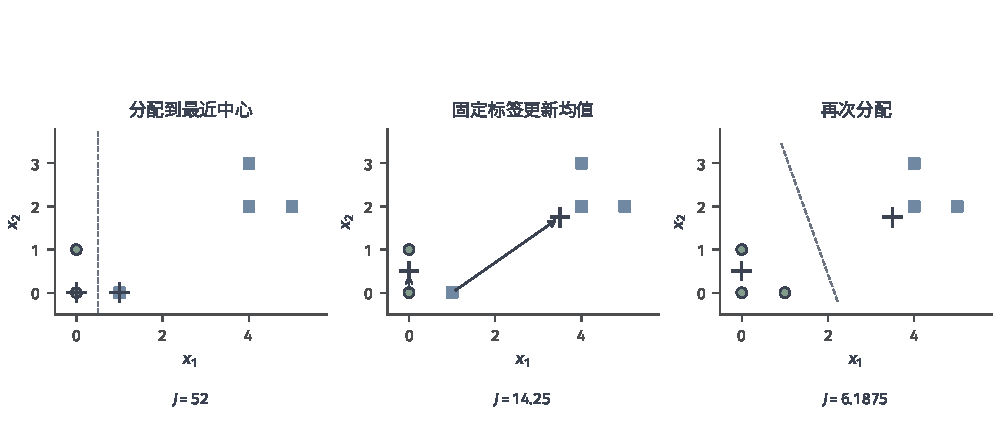
\includegraphics[width=159.059mm]{figures/04-classic-models/00-shared/matplotlib/clustering-lloyd-steps/figure.pdf}
  \caption{Lloyd 迭代的教学例，六个样本为 $(0,0)$、$(0,1)$、$(1,0)$、$(4,2)$、$(4,3)$、$(5,2)$，初始中心为 $(0,0)$ 和 $(1,0)$。圆点与方块表示两个簇，十字表示中心，虚线表示等距边界。首次更新后中心为 $(0,0.5)$ 和 $(3.5,1.75)$；图中依次展示分配、均值更新与再次分配。}
 \label{fig:clustering-lloyd-steps}
\end{figure*}

平局与空簇需要纳入更新规则。等距时优先保留仍属最优的原分配，初始化则按固定顺序决定；空簇没有均值，下面保留其旧中心。这一教学实现最多返回$K$个非空簇。要求恰好$K$个非空簇时，可采用重启或后文的容量约束，并核对相应的停止条件。

\begin{codeblock}[language=Python,label={code:clustering-kmeans}]{带平局与空簇处理的 Lloyd 迭代}
import numpy as np

def kmeans(X, K, max_iter=300, seed=0):
    X = np.asarray(X, dtype=float)
    n = len(X)
    if not 1 <= K <= n or max_iter < 1:
        raise ValueError("invalid K or max_iter")
    rng = np.random.default_rng(seed)
    mu = X[rng.choice(n, K, replace=False)].copy()
    labels = np.full(n, -1)
    for _ in range(max_iter):
        d2 = ((X[:, None] - mu[None]) ** 2).sum(2)
        new = d2.argmin(1)
        rows = np.flatnonzero(labels >= 0)
        keep = d2[rows, labels[rows]] == d2[rows, new[rows]]
        new[rows[keep]] = labels[rows[keep]]
        if np.array_equal(new, labels):
            return labels, mu
        labels = new
        for k in range(K):
            members = X[labels == k]
            if len(members):
                mu[k] = members.mean(0)
    return labels, mu
\end{codeblock}

代码接受有限的二维数值数组。正常停止时，分配与中心形成不动点；迭代上限提前触发时，返回中心已按当前分配更新，但这些分配可能还需再比较一次最近中心。两种退出情形应分别记录。广播计算临时占用$O(nKd)$空间，样本较多时可分块计算距离。

初始中心决定Lloyd从哪里开始搜索。\term{K-means++}先均匀选一个样本，再按$D_i^2/\sum_jD_j^2$抽取后续中心，其中$D_i$是样本到已有中心的最近距离。所有$D_i=0$时，已有中心已覆盖全部不同位置。Arthur与Vassilvitskii证明了初始目标的期望界$\mathbb{E}[J]\leq8(\log K+2)J^\ast$；Lloyd后续不增目标，因此保留这一界\scite{clust-arthur2007}。

该界平均了初始化随机性，单次运行的结果仍可能相差较大。标准K-means++逐个选中心，约需$O(nKd)$运算；分布式实现还需计入数据扫描与通信。评价初始化时，可以同时比较最终平方误差、重启次数和总成本。

\subsubsection{理论分析}

\paragraph{表达能力}
颜色压缩要求用$K$个位置逼近像素分布，因而可以直接用总体平方失真比较候选与目标。只有一个中心时，式\eqref{eq:clustering-mean-decomposition}的总体版本给出
\[
 \inf_{\bm\mu}\mathbb E\lVert\bm X-\bm\mu\rVert_2^2
 =\operatorname{tr}\operatorname{Cov}(\bm X),
\]
条件是输入具有有限二阶矩，最优中心为总体均值。增加中心可以降低这个最小失真；固定$K$时，只有分布集中在至多$K$个位置上，才能把平方失真降为零。例如，将$[0,1]$上的均匀分布用$K$个标量量化，最优中心为等长区间的中点，最小期望失真为$1/(12K^2)$。长度为$\ell$的区间在其中点处贡献$\ell^3/12$，所有区间长度之和为1，凸性使等长划分达到最小值。这个例子明确给出了中心数增加时，模型与量化目标之间还剩多少误差。

客户群组的语义若由另一种关系决定，低失真便未必代表准确分组。比较中心$\bm\mu_a,\bm\mu_b$时，归入前者的条件等价于
\[
 2(\bm\mu_b-\bm\mu_a)^\top\bm x
 \leq\lVert\bm\mu_b\rVert_2^2-\lVert\bm\mu_a\rVert_2^2.
\]
一个簇是这些半空间的交，因而是凸的Voronoi单元。假设目标是把完整的内外同心圆分别分成两簇。包含整个外圆的凸单元必然包含其内部圆盘，不能同时排除内圆；两个中心无论怎样优化，都不能准确表达这个目标。增加中心可以把外圆分成多段，却改变了“一圈一簇”的输出。两片大小或样本比例不同的区域也可能获得不同数量的中心，因为目标按概率质量累加平方失真，并未要求每个语义群体恰用一个中心。Mini-Batch只近似更新相同的中心，不能消除这些表达限制。

\paragraph{收敛性}
Lloyd的有限停止需要目标下降与平局规则共同支持。目标有下界且不增，足以得到目标值的极限；进一步排除无穷次分配变化，才可得到有限轮停止。下面利用有限分配集合完成这一步。

\begin{theorem}[K-means的Lloyd迭代在严格下降条件下的有限停止]
  \label{thm:clustering-lloyd}
  对有限样本，在精确计算下，分配步采用最近中心规则，并在平局时优先保留原簇分配；更新步对非空簇取均值、对空簇保留旧中心。则目标值单调不增，算法在有限轮后到达分配和中心均不再变化的不动点。
\end{theorem}
\begin{proof}
固定中心，逐点选择最小距离给出
\[
 J(\mathcal{P}^{(t+1)},\bm{\mu}^{(t)})
 \leq J(\mathcal{P}^{(t)},\bm{\mu}^{(t)}).
\]
对任意非空簇 $C$，记均值为 $\bar{\bm{x}}_C$。展开平方项，并利用 $\sum_{i\in C}(\bm{x}_i-\bar{\bm{x}}_C)=\bm{0}$，得到
\begin{equation}
 \sum_{i\in C}\lVert\bm{x}_i-\bm{a}\rVert_2^2
 =\sum_{i\in C}\lVert\bm{x}_i-\bar{\bm{x}}_C\rVert_2^2
   +|C|\lVert\bm{a}-\bar{\bm{x}}_C\rVert_2^2.
 \label{eq:clustering-mean-decomposition}
\end{equation}
所以均值是唯一最优中心，更新步也不会增加目标；空簇对目标贡献为零。

第一次均值更新后，若分配改变，至少一个样本移向严格更近的中心，否则保留原标签的规则会阻止改变。因此完整一轮使目标严格下降。对任一分配，均值更新后的目标只由该分配决定，即使存在空簇也如此。分配至多有 $K^n$ 种，严格下降不可能无限次访问它们。分配不变时，已有非空簇中心仍为相同均值，算法遂停止。
\end{proof}

不动点在固定中心时满足最近分配，在固定分配时满足均值最优。若每个样本的最近中心唯一、各簇非空，则足够小的中心扰动保持分配，均值最优性给出局部最优解释。等距样本或重合中心可能破坏这一局部稳定条件，需按退化结构分析。

两个子问题易解，联合的全局搜索仍可能昂贵。维数属于输入时，固定$K=2$的欧氏平方和聚类已是NP-hard\scite{clust-aloise2009}。平面上将$K$作为输入也有NP-hard结果\scite{clust-mahajan2012}。这些结果表明，在$\mathrm{P}\ne\mathrm{NP}$的前提下，一般输入的精确全局解无法统一用多项式时间取得。

\paragraph{泛化性}
学到的中心将怎样处理下一批像素，可以直接用新像素到最近中心的平方距离回答。以下沿用经验风险$\widehat R_n$与期望风险$R$的记号，训练样本$D_n=(\bm X_1,\ldots,\bm X_n)$独立同分布于$P$，风险中的$\bm X\sim P$独立于$D_n$。取$r>0$，将候选中心限制在半径$r$的球内，并假设$\lVert\bm X\rVert_2\leq r$几乎处处成立。此时
\[
 \ell_{\bm\mu}(\bm x)=\min_{1\leq k\leq K}
       \lVert\bm x-\bm\mu_k\rVert_2^2,
 \qquad R(\bm\mu)=\mathbb E_P\ell_{\bm\mu}(\bm X).
\]
这一风险衡量颜色量化失真，尚未涉及簇的语义是否正确。有限样本保证需要同时控制候选中心的数量尺度和求解误差。下面先给出后者如何进入风险界的共同步骤。

\begin{lemma}[有限覆盖下的期望风险界]
 \label{thm:clustering-cover-risk}
取预定的置信参数$\delta\in(0,1)$。
 设$D_n$由$n$个独立同分布观测组成，候选集$\Theta$及其度量在抽样前固定，损失取值于长度为$M$的固定区间，并满足
 $|\ell_\theta(\bm x)-\ell_{\theta'}(\bm x)|\leq L\,d(\theta,\theta')$。
 对任意$\epsilon>0$，设$\Theta$有一个含$N_\epsilon$个点的$\epsilon$覆盖，即每个候选到某个覆盖点的距离至多为$\epsilon$。
 学习器输出$\widehat\theta$，其经验求解误差为
 \[
  e_n=\widehat R_n(\widehat\theta)
          -\inf_{\theta\in\Theta}\widehat R_n(\theta)\geq0.
 \]
 则以至少$1-\delta$的训练抽样概率，
 \begin{equation}
  R(\widehat\theta)-\inf_{\theta\in\Theta}R(\theta)
  \leq4L\epsilon
       +2M\sqrt{\frac{\log(2N_\epsilon/\delta)}{2n}}
       +e_n.
  \label{eq:clustering-cover-risk}
 \end{equation}
 对训练样本及学习器随机性取期望，也有
 \[
  \mathbb E_{D_n}R(\widehat\theta)-\inf_{\theta\in\Theta}R(\theta)
  \leq4L\epsilon
       +2M\sqrt{\frac{\log(2N_\epsilon)}{2n}}
       +\mathbb E_{D_n}e_n.
 \]
\end{lemma}
\begin{proof}
在覆盖点上，Hoeffding界与并集界给出
$\max_\theta|R(\theta)-\widehat R_n(\theta)|
 \leq M\sqrt{\log(2N_\epsilon/\delta)/(2n)}$。
对任意候选，分别将期望风险和经验风险移到最近覆盖点，至多各增加$L\epsilon$，所以全体候选上的偏差至多为
$\Delta_n=2L\epsilon+M\sqrt{\log(2N_\epsilon/\delta)/(2n)}$。
在$R(\widehat\theta)-\inf_\theta R(\theta)$中加入两侧经验风险，得到
$R(\widehat\theta)-\inf_\theta R(\theta)\leq2\Delta_n+e_n$。
期望结论使用同一分解，并对覆盖点的$2N_\epsilon$个带符号偏差应用Hoeffding指数矩界，得到最大偏差的期望至多为
$M\sqrt{\log(2N_\epsilon)/(2n)}$。
\end{proof}

\begin{theorem}[K-means在有界输入下的期望量化风险界]
 \label{thm:clustering-kmeans-risk}
设$D_n$独立同分布于$P$，$\lVert\bm X\rVert_2\leq r$，$r>0$，固定$K$且中心范数至多为$r$。对K-means，损失位于$[0,4r^2]$，用各中心移动距离的最大值衡量两组中心的差异时，$L=4r$。每个$d$维球有至多$(1+2r/\epsilon)^d$个覆盖点，$K$个中心因而有$N_\epsilon\leq(1+2r/\epsilon)^{Kd}$。取$\epsilon=r/n$，式\eqref{eq:clustering-cover-risk}给出
\begin{equation}
 \mathbb E_{D_n}R(\widehat{\bm\mu})
 \leq \inf_{\lVert\bm\mu_k\rVert_2\leq r}R(\bm\mu)
   +\frac{16r^2}{n}
   +8r^2\sqrt{\frac{Kd\log(1+2n)+\log2}{2n}}
   +\mathbb E_{D_n}e_n.
 \label{eq:clustering-kmeans-risk}
\end{equation}
概率至少为$1-\delta$的版本将$\log2$换成$\log(2/\delta)$，并保留实际运行的$e_n$。
\end{theorem}

这里比较的是同一候选中心集中的最佳总体量化误差，无需总体最优中心唯一。中心投影到该球不会增加球内样本的距离，因此这一限制也不损失该设定下的全局最优值。

经验到总体的推理现在有三步：同时控制所有中心的经验偏差，利用学习器在经验目标上的质量，最后比较总体目标。精确经验全局解使$e_n=0$；一次Lloyd或小批量运行只得到局部或近似解，其$e_n$仍须计入，增加样本不能自动消除这一项。Pollard的一致性结果进一步研究最优中心本身的极限\scite{clust-pollard1981}。式\eqref{eq:clustering-kmeans-risk}则直接评价新样本损失。

输入表示同样影响这个损失。平方距离放大远离中心的样本，不同量纲改变最近中心的次序，因此尺度选择需对应业务含义。第\ref{sec:regression-knn}节的$k$-NN回归也依赖距离，但它平均带响应的邻居，K-means拟合无标签输入的位置。

\subsubsection{优化表达能力}

中心分配的形状也受表示限制。考虑围绕同一圆心的内外两圈样本，两圈的均值都靠近圆心，用两个原空间中心难以按半径分开它们。若以半径平方作为一个新特征，内外圈在该坐标上就落在不同位置。\term{核 K-means}（kernel K-means）采用相同思路，在特征映射$\phi$之后比较样本与簇均值。第\ref{sec:classic-overview-kernel-trick}节的正定核$K$允许我们直接计算这些距离；映射是否适合当前群组，仍由核的选择决定。样本到簇均值的平方距离为
\begin{equation}
 \begin{aligned}
 \lVert\phi(\bm{x}_i)-\bm{\mu}_k^\phi\rVert^2
 ={}&K(\bm{x}_i,\bm{x}_i)
 -\frac{2}{|C_k|}\sum_{j\in C_k}K(\bm{x}_i,\bm{x}_j)\\
 &+\frac{1}{|C_k|^2}
   \sum_{j,l\in C_k}K(\bm{x}_j,\bm{x}_l).
 \end{aligned}
 \label{eq:clustering-kernel-kmeans}
\end{equation}
公式只使用核值，省去了显式构造$\phi$，相应成本转为核矩阵计算与存储\scite{clust-girolami2002,dhillon2004}。Girolami讨论核空间聚类，Dhillon、Guan与Kulis进一步联系了适当权重和核构造下的核K-means与归一化割。

同心圆的例子可以核验映射带来的收益。对半径分别为$r_1,r_2$的两个完整圆，取$\phi(\bm x)=\lVert\bm x\rVert_2^2$，对应的正定核为$K(\bm x,\bm y)=\lVert\bm x\rVert_2^2\lVert\bm y\rVert_2^2$。两圈分别变为标量$r_1^2,r_2^2$，用两个中心可得到零特征失真，并准确保留“一圈一簇”。若两组半径存在重叠，仅保留这个特征就无法区分重叠位置；若目标按角度分组，它还会把同半径的不同群组混在一起。核技巧让特定非线性关系进入候选范围，效果需要对应目标，而不能由“采用了核”单独保证。

核K-means与归一化割的联系依赖适当的权重和核构造，适用范围需随具体等价关系核对。特征映射可以改变原空间的分配形状，层次结构则改变输出粒度；多层输出见第\ref{sec:clustering-hierarchy}节，局部密度与连接提供了另一种描述弯曲群组的方式。

\subsubsection{优化泛化能力}

中心的选择还取决于怎样评价距离。用一个固定簇的单坐标教学例子看：数据为$0,0,0,100$时，平方距离和在均值$25$处最小，绝对距离和则在中位数$0$处最小。极端记录可以把均值拉离多数样本，改用绝对距离就改变了这种牵动。\term{K 中位数聚类}（K-medians）最小化$\ell_1$距离和，固定分配后逐坐标取中位数；它不等于以欧氏距离和定义的几何中位数问题。

在这个例子中，单中心的最小绝对距离和为100，而在均值25处为150；反过来，中位数处的平方距离和为10000，均值处为7500。因而改用中位数改善的是绝对距离目标，不能据此宣称对平方量化也更准确。多维$\ell_1$损失逐坐标相加，适合目标确实要求累加各坐标绝对偏差的情形；它没有利用坐标间的相关方向，也没有为弯曲群组增加新的连接表示。

\subsubsection{优化计算能力}

颜色压缩若涉及大量图像，一次中心更新就要重新比较全部像素与$K$个中心，即使中心只移动一点，也要付出一次全量扫描的成本。\term{小批量K均值聚类}（Mini-Batch K-means）改用抽取的$b$个样本估计更新方向，只调整这些样本涉及的中心。Sculley在2010年研究了这一方法\scite{clust-sculley2010}。平方距离目标仍然保留，每轮采用的信息量与计算量则减少了。

设簇 $k$ 累计接收了 $v_k$ 次样本更新。每接收一个分配到该簇的样本，就令 $v_k\leftarrow v_k+1$，并计算
\begin{equation}
 \bm{\mu}_k\leftarrow
 (1-\eta_k)\bm{\mu}_k+\eta_k\bm{x}_i,
 \qquad \eta_k=\frac{1}{v_k}.
 \label{eq:clustering-minibatch}
\end{equation}
这是对历史已分配样本的增量平均，不是当前全体簇成员的精确均值。一轮距离计算降为 $O(bKd)$，但总成本仍取决于迭代次数、初始化和最终全量分配。

随机小批量使每次更新只反映部分样本，逐轮全量SSE可能波动。批量大小、采样偏差和低频簇的覆盖影响最终误差；定理~\ref{thm:clustering-lloyd}针对完整分配与精确均值更新，其单调性前提在这里发生改变。选择计算预算时，应以抽样评价或留出量化误差检查这种近似是否足够。

\subsubsection{支持簇容量约束场景}

\label{sec:clustering-capacity}

用于服务网点分配时，最近中心规则还可能违反容量要求。假设一个网点最多服务100条客户记录，它附近却有150条记录；把这些记录全部分给最近网点可以减小SSE，却使方案无法执行。限制簇大小的方法把每簇的最小与最大容量加入分配条件，再在可行方案中比较距离。Bradley、Bennett与Demiriz研究了带最小簇规模的K-means；加入上界后，固定中心的分配问题可统一写为\scite{clust-bradley2000}。
\begin{equation}
 \begin{aligned}
 \min_{\bm{Z}}\quad&
   \sum_{i=1}^n\sum_{k=1}^K
   z_{i,k}\lVert\bm{x}_i-\bm{\mu}_k\rVert_2^2,\\
 \text{s.t.}\quad&
   \sum_{k=1}^K z_{i,k}=1,\quad z_{i,k}\in\{0,1\},\\
 & \ell_k\leq\sum_{i=1}^n z_{i,k}\leq u_k.
 \end{aligned}
 \label{eq:clustering-capacity}
\end{equation}
整数容量满足 $0\leq\ell_k\leq u_k$，且在没有其他分配禁令时，可行性条件为 $\sum_k\ell_k\leq n\leq\sum_ku_k$。

固定中心的容量分配可转为最小费用流。源点到每个样本的边容量为1，样本到每簇的边容量为1、费用为平方距离，簇到汇点的边下界为$\ell_k$、上界为$u_k$，总流量为$n$。网络流的整数性保证存在整数最优解，使每个样本恰好选择一簇；这一性质来自网络约束的结构。

容量方法的中心仍按均值更新。每次分配精确最优且平局保留已有最优分配时，分配变化导致严格下降；采用确定的空簇处理后，可按有限分配集合证明停止。求解成本取决于网络规模、费用表示与求解器，需按具体实现估计。

Malinen 与 Fränti 在 2014 年研究了要求簇规模相等的平衡 K-means\scite{clust-malinen2014}。当 $K$ 整除 $n$ 且要求 $|C_k|=n/K$ 时，把每个中心复制成相应数量的容量槽，得到 $n$ 对 $n$ 的指派问题；Hungarian 算法可在 $O(n^3)$ 时间内求解。

当$n$不能被$K$整除，可为各簇指定$\lfloor n/K\rfloor$或$\lceil n/K\rceil$个槽，并使容量总和为$n$。按距离顺序填槽可以节省搜索，却可能让先处理的样本占用后续样本所需位置。使用这种启发式时，还需检查全部下界与实际SSE变化。

容量约束表达的是一批对象共同满足的分配要求。若目标方案满足给定上下界，它仍在候选范围内；若一个目标簇有150条记录而上界为100，这个簇就必须拆开或让部分记录转组。受约束的最小SSE不小于无约束的最小SSE，增加的失真是满足容量的代价。此时一个样本的归属取决于其他样本占用了哪些槽，不能再把训练划分解释成独立的最近中心区域。对新的一批客户执行相同容量要求，还需要共同求解分配。

\subsubsection{支持模糊隶属度输出场景}

最近中心规则只给出一个簇标签，无法表达样本处于两个群组之间的程度。例如，一位客户的购买行为同时接近两类典型客户，略微改变记录就可能使硬标签跳到另一类。\term{模糊 C 均值}（Fuzzy C-Means, FCM）保留各中心之间的比较，用隶属度$u_{i,k}$分配软归属，因而可以表达这种过渡\scite{clust-bezdek1981}。
\begin{equation}
 J_{\mathrm{FCM}}
 =\sum_{i=1}^n\sum_{k=1}^K
 u_{i,k}^{q}\lVert\bm{x}_i-\bm{\mu}_k\rVert_2^2,
 \quad \sum_k u_{i,k}=1,\quad q>1.
 \label{eq:clustering-fcm}
\end{equation}
这里$q$控制隶属度的模糊程度。固定隶属度时，中心是以 $u_{i,k}^q$ 为权重的均值；当各距离非零时，固定中心给出
\[
 u_{i,k}=
 \left[
 \sum_{j=1}^K
 \left(\frac{\lVert\bm{x}_i-\bm{\mu}_k\rVert_2}
 {\lVert\bm{x}_i-\bm{\mu}_j\rVert_2}\right)^{2/(q-1)}
 \right]^{-1}.
\]
若样本与一个或多个中心重合，可把隶属度集中在这些零距离中心上。隶属度表示模糊目标下的软归属；赋予生成后验含义还需要相应概率模型。医学影像中一个像素混合多种组织的部分体积效应，可为这种软表达提供应用动机。

FCM能够表达的软关系仍由中心距离约束。两个距离相等且非零时，两者的隶属度相等；所有$K$个距离相等时，各隶属度必为$1/K$。若两类在该位置的真实比例并不相等，仅调$q$不能让这个规则给出所需比例，因为$q$只改变距离比的指数。对内外同心圆，若两个中心都取圆心，两圈上的每个点都会得到相同的均匀隶属度，无法表示半径决定的成分归属。软输出补充了边界过渡，却没有自动补充形状或生成比例。

\subsubsection{支持层次划分输出场景}

若除了最终的$K$组，还希望看到“先分成哪两大组，再怎样细分”，一次性$K$中心划分没有保留这种关系。\term{二分 K-means}（Bisecting K-means）从全部样本组成的一簇开始，反复选择一个簇作$K=2$划分。常见实现选择最大SSE的簇，并为每次二分多次重启。分裂记录形成一棵层次树，但早期分开的对象以后不能跨分支重组，最终SSE因而不保证优于一次性$K$分。Steinbach等在文档聚类中研究了这一方案\scite{clust-steinbach2000}。

每次最近双中心分裂都增加一个半空间条件，最终叶簇是沿路径得到的半空间交，仍为凸区域。它可以表示不同粒度下相互包含的群组；若某个目标群组跨越了早期切面，后续细分只能把它切成更多片，不能重新组成一簇。因此，层次输出增加了可解释的粒度关系，并未消除原空间中心划分对环形目标的限制。

\subsubsection{小结}

K-means适合把数值记录压缩成有限个中心，平方距离规定了怎样比较压缩误差。使用前应先确定各坐标的尺度与$K$的含义：用于颜色量化时，中心代表可用颜色；用于客户分析时，最近中心形成的群组还需要业务证据解释。

围绕同一个平方误差目标，可以分别调整计算与可行分配。小批量更新只访问部分记录，节省每轮扫描，但需要检查低频簇的覆盖与最终失真。容量约束把“网点能接收多少客户”写入分配问题，得到可执行的方案，同时增加共同分配的求解成本，并可能增加距离损失。

其他调整改变了所要表达的群组。绝对距离减弱极端记录对中心位置的牵动，FCM允许边界样本软归属，二分方案保留层次，核表示则改变比较样本的坐标。它们分别改变损失、输出粒度或表示，不能互相替代：软标签未消除单中心的形状限制，核映射也需要保留任务所需的区别。

\subsection{K-medoids}
\label{sec:clustering-kmedoids}

均值适合数值量化，却未必适合展示一个群组的典型对象。客户各项特征的平均值可能不对应任何真实客户；字符串之间可以计算编辑距离，却不能像数值向量一样取均值。\term{K 中心样本聚类}（K-medoids）把代表限制为已有样本，选择使组内总相异度较小的真实对象。这样既能展示一条可以核查的代表记录，也能直接使用字符串等对象的相异度；代价是需要在候选样本之间搜索代表。

Kaufman与Rousseeuw在1987年介绍了通过medoid聚类的方法，以真实观测作代表，使相异度矩阵能够直接作为输入\scite{clust-kaufman1987}。1990年的专著进一步整理了PAM、面向较大数据的CLARA及层次分析\scite{clust-kaufman1990}。代表的解释与候选代表的搜索由此成为两个独立的设计问题。

\subsubsection{模型结构}

设代表索引集合 $M=\{m_1,\ldots,m_K\}\subseteq\{1,\ldots,n\}$，相异度为 $\delta(\bm{x},\bm{y})$。优化目标为
\begin{equation}
 J(M)=\sum_{i=1}^n\min_{m\in M}\delta(\bm{x}_i,\bm{x}_m).
 \label{eq:clustering-medoids}
\end{equation}
每个 $\bm{x}_{m_k}$ 称为\term{中心样本}（medoid），分配由最近代表决定。典型相异度包括欧氏距离、曼哈顿距离、汉明距离、编辑距离和 Jaccard 距离。目标本身不要求三角不等式，但某些索引加速方法需要这一性质。

未平方距离随远点的偏移增长较慢，真实样本约束也改变了中心的可移动范围，两者可减弱极端值对SSE均值的影响。具体鲁棒性仍由相异度和污染位置决定：离群点若改变候选代表的相对距离，也可能改变medoid。

图~\ref{fig:clustering-medoid-robustness}固定一维单簇，将最右样本由5移到12。平方距离的最优中心随均值右移，绝对距离的最优中心样本仍为中间观测2。该对照同时改变损失与代表约束，结论限于这组设定；它提供了检查极端值影响的可核算例子。

\Needspace{75mm}
\begin{figure}[htbp]
  \centering
  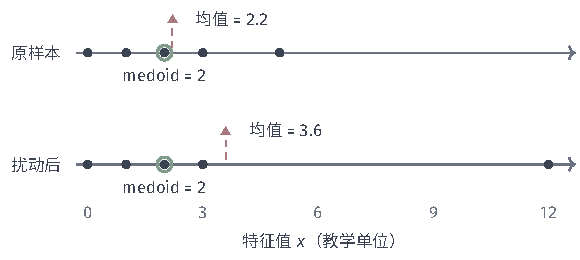
\includegraphics[width=98.231mm]{figures/04-classic-models/00-shared/tikz/clustering-medoid-robustness/figure.pdf}
  \caption{中心样本与均值对极端值的不同反应。固定 $K=1$，上方样本为 $\{0,1,2,3,5\}$，下方只把 5 改为 12；黑点为观测，圆圈标出绝对距离下的 medoid，三角形标出平方距离下的最优均值。}
 \label{fig:clustering-medoid-robustness}
\end{figure}

\subsubsection{参数学习}

\term{围绕中心样本划分}（Partitioning Around Medoids, PAM）通常包含 BUILD 初始化和 SWAP 改进。BUILD 贪心增加代表；SWAP 枚举每个当前代表 $m\in M$ 与每个非代表 $o\notin M$，计算
\[
 \Delta(m,o)=
 J\bigl((M\setminus\{m\})\cup\{o\}\bigr)-J(M).
\]
候选 $o$ 来自整个数据集，而不限于 $m$ 所在簇；每次交换后，所有样本都重新选择最近代表。只在固定簇内选取距离总和最小的样本，是另一种交替更新，不能替代 PAM 的 SWAP。

下面从随机代表开始，逐个评价完整交换邻域，以便核对$J(M)$与返回状态。代码省略BUILD初始化和距离差分缓存，适合作为目标及停止判据的教学实现。

\begin{codeblock}[language=Python,label={code:clustering-pam}]{PAM 的完整交换步骤}
import numpy as np

def pam_swap(D, K, seed=0, max_iter=100):
    n = len(D)
    if D.shape != (n, n) or not 1 <= K <= n or max_iter < 1:
        raise ValueError("invalid distance matrix, K, or max_iter")
    rng = np.random.default_rng(seed)
    medoids = rng.choice(n, K, replace=False)
    cost = D[:, medoids].min(1).sum()
    converged = False
    for _ in range(max_iter):
        best, best_cost = None, cost
        outside = np.setdiff1d(np.arange(n), medoids)
        for k in range(K):
            for o in outside:
                trial = medoids.copy()
                trial[k] = o
                value = D[:, trial].min(1).sum()
                if value < best_cost:
                    best, best_cost = trial, value
        if best is None:
            converged = True
            break
        medoids, cost = best, best_cost
    return D[:, medoids].argmin(1), medoids, converged
\end{codeblock}

完整扫描若未发现改进交换，代码返回\code{converged=True}，表明当前代表集合在单次交换邻域中局部最优。迭代上限先触发时，\code{converged=False}保留了尚未核完下一邻域的状态。严格下降使代表集合不重复，去掉上限并继续扫描时，有限候选集合保证最终停止。

预计算相异度矩阵占用$O(n^2)$存储，距离本身的计算还需另外计入。经典PAM缓存最近与次近代表，一轮完整交换通常按$O(K(n-K)^2)$量级分析。教学代码为每个候选重算$K$个距离列，额外重复了这些访问，因此成本更高。

\subsubsection{理论分析}

\paragraph{表达能力}
以欧氏距离作相异度时，K-medoids同样按最近代表分组，距离是否平方不改变两代表之间的等距边界。因此，前述内外同心圆不能由两个单一代表准确分开的限制仍然存在；换成真实样本并没有改变这一几何关系。改用编辑距离或图距离后，候选分组可以利用相应对象关系，但能否吻合目标要由该相异度决定，欧氏凸单元的结论也不再适用。

将代表限制在输入支持上，也可能使最小量化距离大于不受这一约束时的距离。以单位圆上均匀分布的输入和$K=1$为教学例，若允许任意欧氏位置作代表，圆心使期望距离达到最小值1；凸性与旋转对称性保证圆心最优。若代表必须是圆上的观测，则无论选择哪一点，期望距离都为
\[
 \frac1{2\pi}\int_0^{2\pi}2|\sin(\theta/2)|\,\mathrm d\theta
 =\frac4\pi.
\]
两者相差$4/\pi-1$。这种差异来自候选代表只能落在输入支持上，而非PAM没有搜索充分。若只允许代表来自输入支持的更小子集，候选空间进一步缩小，最小量化距离不会降低。



\paragraph{收敛性}
固定$K$时，样本代表集合至多有$\binom nK$种，因而最优集合存在。若每次交换都严格降低同一目标，已经访问的集合不能再次出现，至多接受$\binom nK-1$次交换后便会停止。PAM完整扫描没有改进时，得到的是单次交换意义下的局部最优；这个有限性上界很粗，也没有把局部解提升为全局解。

\paragraph{泛化性}
采用欧氏距离时，冻结代表后可以评价新样本的平均最近代表距离。

\begin{theorem}[K-medoids在有界欧氏输入下的期望量化风险界]
 \label{thm:clustering-medoids-risk}
设$D_n$独立同分布于$P$，$\lVert\bm X\rVert_2\leq r$，所有原型也在该球内。损失
$\ell_{\bm m}(\bm x)=\min_k\lVert\bm x-\bm m_k\rVert_2$
位于$[0,2r]$，原型最多移动$\epsilon$时损失最多改变$\epsilon$。沿用引理\ref{thm:clustering-cover-risk}的覆盖计算，得到
\begin{equation}
 \mathbb E_{D_n}R(\widehat{\bm m})
 \leq\inf_{\lVert\bm m_k\rVert_2\leq r}R(\bm m)
   +\frac{4r}{n}
   +4r\sqrt{\frac{Kd\log(1+2n)+\log2}{2n}}
   +\mathbb E_{D_n}e_n.
 \label{eq:clustering-medoids-risk}
\end{equation}
\end{theorem}

这里$e_n$按整个球中的原型计算，因此既含PAM等算法的搜索误差，也含代表只能来自样本的限制。即使完整求出最佳medoid，也不能直接令这个$e_n$为零。若用任意相异度，并预先固定$J$个候选代表、限制损失于$[0,M]$，则候选数至多为$J^K$，对应的超额风险界为
$2M\sqrt{[K\log J+\log(2/\delta)]/(2n)}+e_n$，概率至少为$1-\delta$。候选库由同一训练集生成时，不满足这个固定有限库的条件，需另作复杂度分析。

\subsubsection{优化计算能力}

完整交换邻域昂贵时，可以减少候选代表或减少检查的交换。Kaufman与Rousseeuw整理的CLARA在若干子样本上运行PAM，再用全体样本评价候选代表，以减少工作集；抽样未覆盖的小簇可能因此没有合适代表。Ng与Han在1994年提出的CLARANS把代表集合视为状态，随机抽取交换邻居，减少每轮扫描量\scite{clust-nghan1994}。前者限制本轮代表从哪里来，后者限制本轮搜索哪些交换，两者都需要评价近似搜索的损失。

重复计算也可以在保留交换目标的前提下减少。Schubert与Rousseeuw在2019年的FastPAM工作中复用不同被替换代表之间的计算，减少经典SWAP中随$K$重复的工作\scite{clust-schubert2019}。这种改进主要针对交换评价；关于$n$的距离访问和全量矩阵存储仍需计入，大样本的瓶颈可能继续来自这两部分。

\subsubsection{小结}

K-medoids以真实记录代表群组，可以解释典型对象，也能接收无法取均值的字符串等相异度输入。代表必须来自样本是一项实际约束，指定相异度又规定了哪些对象算作相近；极端值是否影响代表，需结合这两项选择判断。

搜索成本较高时，CLARA通过抽样缩小候选来源，CLARANS只检查部分交换，FastPAM则复用交换计算。前两者可能遗漏重要代表或改进机会，后一类加速仍需承担距离访问与存储。若连代表数也不想预先固定，第\ref{sec:clustering-affinity-propagation}节的AP提供另一种消息搜索路线，但同时改用偏好参数控制代表选择，不能当作PAM的等价加速。

\subsection{模型对比与总结}

原型方法共同用少量代表概括一批对象。K-means允许代表在向量空间中移动，平方欧氏距离使固定分组的最优代表可以直接取均值，更新成本较低。需要展示真实客户、典型文档或其他无法取均值的对象时，这个代表约束就不够：K-medoids改从观测中选代表，并允许采用指定相异度，代价是要搜索代表交换。表~\ref{tab:clustering-partition}比较这两个变化；采用真实代表也不自动带来鲁棒性，还需检查相异度对极端记录怎样计价。

\begin{table}[htbp]
 \small
 \begin{tabularx}{\linewidth}{@{}l>{\RaggedRight\arraybackslash}X>{\RaggedRight\arraybackslash}X@{}}
 \toprule
 比较项 & K-means & K-medoids\\
 \midrule
 代表 & 簇内均值向量 & 真实样本\\
 准则 & 平方欧氏距离和 & 指定相异度和\\
 优化步骤 & 最近中心与均值更新 & 代表交换与全局重分配\\
 主要成本 & 一轮 $O(nKd)$ & 完整交换搜索与距离访问\\
 典型用途 & 数值数据、向量量化 & 非数值对象、实例解释\\
 \bottomrule
 \end{tabularx}
 \caption{两类划分方法的比较。复杂度须与具体算法相联系；PAM 的成本不能套到所有 K-medoids 求解器。}
 \label{tab:clustering-partition}
\end{table}

围绕中心表示，损失和输出可以分别调整。K-medians把平方偏差换成绝对偏差，减弱少量极端记录对中心位置的牵动；FCM保留多个中心的软归属，表达边界过渡；核K-means改变比较坐标，使适当的非线性关系进入最近中心表示。前两者没有消除原空间单中心的形状限制，核方法也没有自动获得所需核。容量约束与二分层次则分别改变可行分配和输出粒度，回应了另一类使用要求。

数据规模主要影响怎样求解这些目标。Mini-Batch K-means用随机记录近似中心更新，CLARA限制代表搜索的工作集，CLARANS抽查交换机会；它们用近似换取较少访问。FastPAM则复用交换统计，减少同一搜索中的重复工作。选择时应同时核对失真、代表是否真实、重要小簇是否被抽样覆盖及资源预算，不能只把这些方法都归为“快速聚类”。

\section{基于邻域的聚类}
\label{sec:clustering-density}

环形、月牙形和弯曲条带中的样本可能远离同一中心，却能沿密集区域连接。密度方法据此把低密度分隔加入簇定义：一类方法寻找密集区域的连通分量，另一类寻找密度峰的吸引域。同一连通区域可以包含多个峰，因此两种定义会产生不同划分。

DBSCAN 直接用邻域计数判断密集程度，OPTICS 保留不同密度尺度的访问结构，Mean Shift 则沿核密度估计寻找驻点。噪声识别是前两者的显式输出；基本 Mean Shift 会为起点寻找归宿，并不自动拒绝孤立样本。

\subsection{DBSCAN}
\label{sec:clustering-dbscan}

考虑两条彼此分开的弯曲点带。沿同一条带相邻的样本很近，带的两个端点却可能很远；最近中心分配用到中心的距离，容易把一条带切开。若再有几个孤立点，K-means仍会把它们分进某个簇。DBSCAN（Density-Based Spatial Clustering of Applications with Noise）改用局部邻居的数量判断哪些位置足够密集，再沿相连的密集邻域扩展。只要两条带内部连通、带间没有密集路径，它们就可以各自形成一簇，孤立点则保留为噪声。Ester等在1996年提出了这一方法\scite{ester1996}。

原始DBSCAN面向带噪声的大型空间数据库，将任意形状的密集区域、参数知识需求和处理成本列为设计问题。邻域计数决定哪些点能扩展，连通搜索把它们组织成簇，无法归属的点保留噪声标记。这样，簇的数量和拒绝范围由局部密度关系共同确定。

\subsubsection{模型结构}

固定半径 $\varepsilon>0$ 和最小邻域样本数 $m=\mathrm{MinPts}$，定义索引邻域
\[
 N_\varepsilon(i)=
 \{j:\delta(\bm{x}_i,\bm{x}_j)\leq\varepsilon\}.
\]
本节假定相异度对称、样本到自身距离为零，并在邻域计数中包含自身。\term{核心点}（core point）满足 $|N_\varepsilon(i)|\geq m$；\term{边界点}（border point）不是核心点，但处在某个核心点的邻域内；既非核心也非边界的样本是\term{噪声点}（noise point）。

若 $i$ 是核心点且 $j\in N_\varepsilon(i)$，称 $j$ 从 $i$\term{直接密度可达}（directly density-reachable）。沿这样的有向关系组成有限链，就得到\term{密度可达}（density-reachable）：链上除终点外的点都须为核心点，终点可以是边界点。若存在一个核心点，使两个样本都从它密度可达，则称它们\term{密度相连}（density-connected）。

先只看核心点邻接图，可以清楚地区分扩展与吸收：距离不超过$\varepsilon$的核心点相连，每个连通分量提供一个簇的核心，再吸收相邻非核心点。边界点可能同时邻接多个分量；实际DBSCAN通常交给先访问它的簇，从而得到单一标签。图~\ref{fig:clustering-dbscan}展示了核心点继续扩展、边界点只被吸收的差别。

\begin{figure}[htbp]
  \centering
  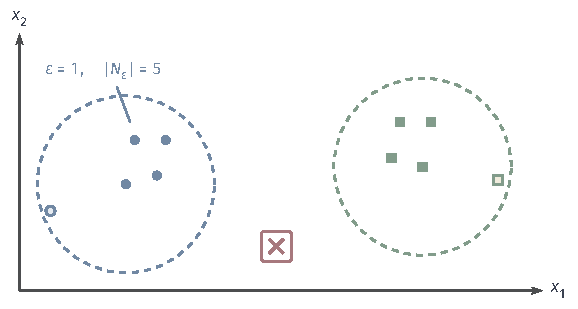
\includegraphics[width=97.850mm]{figures/04-classic-models/00-shared/tikz/clustering-dbscan/figure.pdf}
  \caption{DBSCAN的教学示意，取$\varepsilon=1$、$\mathrm{MinPts}=4$，计数包含自身。圆形和方形分别标识两个核心分量，颜色只作辅助；实心标记为核心点，浅色填充标记为边界点，红框叉号为噪声。虚线圆表示两个示例核心点的邻域；左侧标注直接给出邻域内计数，边界点不能继续扩展簇。}
 \label{fig:clustering-dbscan}
\end{figure}

\subsubsection{参数学习}

DBSCAN 的主要工作是查询邻域并搜索核心连通分量。代码~\ref{code:clustering-dbscan} 使用暴力距离查询，完整展示暂定噪声被重新吸收为边界点的情况。

\begin{codeblock}[language=Python,label={code:clustering-dbscan}]{DBSCAN 的邻域扩展}
import numpy as np
from collections import deque

def dbscan(X, eps, min_pts):
    X = np.asarray(X, dtype=float)
    if eps <= 0 or min_pts < 1:
        raise ValueError("invalid density parameters")
    labels = np.full(len(X), -1)  # -1 未访问，-2 噪声
    def neighbors(i):
        d2 = ((X - X[i]) ** 2).sum(1)
        return np.flatnonzero(d2 <= eps ** 2)
    cid = 0
    for i in range(len(X)):
        if labels[i] != -1:
            continue
        near = neighbors(i)
        if len(near) < min_pts:
            labels[i] = -2
            continue
        labels[i] = cid
        queue = deque(near)
        while queue:
            j = queue.popleft()
            if labels[j] == -2:
                labels[j] = cid
            if labels[j] != -1:
                continue
            labels[j] = cid
            near_j = neighbors(j)
            if len(near_j) >= min_pts:
                queue.extend(near_j)
        cid += 1
    return labels
\end{codeblock}

代码中每个样本至多查询一次邻域，队列则可能保存重复索引。暴力距离计算约需$O(n^2d)$运算。低维数据且邻域规模受控时，空间索引可使实践成本接近$O(n\log n)$；高维或大半径会增加访问量，最坏仍可达到平方级。预存全部邻域还可能占用$O(n^2)$内存。

参数选择可从第 $m$ 近邻距离的排序图入手，近邻计数约定应与是否包含自身一致。曲线的转折提示不同密度尺度，但未必存在清晰肘部。Schubert 等把 $\mathrm{MinPts}\approx 2d$ 作为平滑密度估计的经验起点，而不是一般最优值\scite{clust-schubert2017}。重复样本、噪声比例和有效维数都会影响合理的邻域大小与最小样本数。

\subsubsection{理论分析}

\paragraph{表达能力}
DBSCAN可以把一整条弯曲点带表示为一簇，因为同簇条件要求沿局部邻域连通，并不要求所有点都靠近一个中心。具体而言，假设目标划分中的每个点都有至少$m$个$\varepsilon$邻居，每个目标簇内部的$\varepsilon$邻接图连通，且不同目标簇之间的点距都大于$\varepsilon$。所有点此时都是核心点，核心图的连通分量恰与目标簇相同，DBSCAN便能完整表达该划分。条件中没有凸性要求，因此也适用于满足这些邻接条件的环形或月牙形样本。

同一机制也明确限定了哪些目标不能表达。两条点带之间若出现核心点组成的$\varepsilon$路径，DBSCAN就必须把它们合并，即使任务要求它们分开；若稀疏带上的点都不足$m$个邻居，它们就不能形成自己的核心簇。增大半径可以补足稀疏带的邻居，却可能同时连接稠密区域。这不是搜索精度不足，而是固定$(\varepsilon,m)$定义的候选分组与目标冲突。边界点还只能吸附到核心簇，若目标希望把一批彼此相近、却不邻接任何核心点的记录单独保留为簇，该参数下也无法做到。

\paragraph{收敛性}
DBSCAN的访问和扩展在有限样本上结束，其计算任务是搜索核心连通分量。由于这里没有连续参数的迭代优化，需要验证的是搜索是否完整，以及固定数据下哪些输出与访问顺序无关。

\begin{lemma}[DBSCAN 的核心点确定性]
 \label{thm:clustering-dbscan}
 固定数据、对称相异度和参数 $(\varepsilon,m)$，DBSCAN 输出的每个簇限制到核心点后，恰为核心点邻接图的一个连通分量。因此核心点划分与访问顺序无关，簇编号的置换除外。
\end{lemma}
\begin{proof}
在核心点集合上，距离不超过 $\varepsilon$ 的两点能相互直接密度到达。有限链的连通关系满足自反、对称和传递性，故图的连通分量就是核心点上密度相连关系的等价类。

从任一尚未访问的核心点扩展时，每发现一个核心邻居就加入它的邻域。沿路径长度归纳，该点所在连通分量中的每个核心点最终都会被访问。反过来，扩展过程只能经由核心点邻接边到达其他核心点，不能穿过非核心边界点连接两个分量。因此输出的核心集合既不遗漏本分量，也不包含其他分量，结论成立。
\end{proof}

定理固定了核心点划分。一个边界点若邻接多个核心分量，其单一归属仍由访问规则决定；簇编号和共享边界归属是两种不同的顺序影响。

\paragraph{泛化性}
DBSCAN的连通分量属于当前样本，加入新点可能改变核心计数并连接原先分开的分量。固定数据的搜索正确性因此不能直接给出新样本分组的期望风险。不过，核心判定本身可以先作为一个明确的总体任务来分析。

\begin{theorem}[DBSCAN在邻域质量间隔条件下的期望核心判定风险界]
 \label{thm:clustering-dbscan-core-risk}
设$D_n$独立同分布于$P$，新点独立于训练集。固定半径$\varepsilon$及质量阈值$t\in(0,1)$，记
$p_\varepsilon(\bm x)=P\{\delta(\bm x,\bm X)\leq\varepsilon\}$。
总体核心规则为$c_\star(\bm x)=\mathbf1\{p_\varepsilon(\bm x)\geq t\}$，训练后冻结的规则为
$\widehat c_n(\bm x)=\mathbf1\{n^{-1}\sum_i\mathbf1\{\delta(\bm x,\bm X_i)\leq\varepsilon\}\geq t\}$。
这里新点不计入训练邻居；$t$对应查询所用的计数阈值除以$n$。
若存在$\gamma>0$使$P\{|p_\varepsilon(\bm X)-t|\geq\gamma\}=1$，则新点的核心判定风险满足
\begin{equation}
 \mathbb E_{D_n}\!\left[
   P_{\bm X}\{\widehat c_n(\bm X)\ne c_\star(\bm X)\mid D_n\}
 \right]\leq2e^{-2n\gamma^2}.
 \label{eq:clustering-dbscan-core-risk}
\end{equation}
\end{theorem}

对每个固定查询$\bm x$，邻居指示量独立且均值为$p_\varepsilon(\bm x)$；越过判定阈值至少需要$\gamma$的计数偏差。Hoeffding界控制这一概率，再对独立新点积分，即得该式。没有统一间隔时，对任意$\gamma>0$仍有上界
$P\{|p_\varepsilon(\bm X)-t|<\gamma\}+2e^{-2n\gamma^2}$，阈值附近的概率质量成为额外误差。

这个结论只保证固定尺度下的核心判定，不保证连通簇与语义类别一致。要评价簇标签，必须另定总体簇、核心分量的匹配、新点分配以及冲突和拒绝规则；新增点重跑搜索也改变了学习器。OPTICS与HDBSCAN保留更多尺度，所选阈值若由同一批数据决定，也需另控制选择误差。

\subsubsection{小结}

DBSCAN由局部计数产生核心点，再以连通性形成簇，并显式保留噪声。它省去预设$K$，同时引入全局半径、计数阈值及距离选择。可恢复的形状由密度连通定义决定，高维查询和不同密度群组仍可能限制实际效果。

\subsection{OPTICS}
\label{sec:clustering-optics}

前述两条点带如果疏密不同，DBSCAN的单一半径就不容易选择：半径较小会拆散稀疏带，较大又可能把原本应分开的稠密区域连起来。反复换半径还会重复查询相似邻域。OPTICS（Ordering Points To Identify the Clustering Structure）在一次搜索中保存样本次序及进入相邻密集区域所需的距离，让我们事后查看不同尺度下的连接变化。Ankerst等在1999年提出的方法先给出这些记录，再由提取规则得到划分\scite{clust-ankerst1999}。

OPTICS把邻域计算与划分提取分开。DBSCAN在给定尺度后返回簇标签，OPTICS先保存访问次序和距离，供后续比较多种尺度。探索密度群组因而主要转为读取同一份结果，同时需要明确采用的提取规则。

\subsubsection{模型结构}

设搜索半径上限为 $\varepsilon_{\max}$。若样本 $i$ 在该半径内有至少 $m$ 个邻居，则其\term{核心距离}（core distance）为第 $m$ 近邻距离；否则记为 $+\infty$：
\[
 a_i=
 \begin{cases}
 \delta_{i,(m)},&|N_{\varepsilon_{\max}}(i)|\geq m,\\
 +\infty,&\text{其他情况}.
 \end{cases}
\]
由核心点 $i$ 到邻居 $j$ 的\term{可达距离}（reachability distance）定义为
\begin{equation}
 r(j\mid i)=\max\{a_i,\delta(\bm{x}_i,\bm{x}_j)\}.
 \label{eq:clustering-reachability}
\end{equation}
方向来自出发点的核心距离，因此通常 $r(j\mid i)\ne r(i\mid j)$。它表示在确保出发点足够密集的同时覆盖 $j$ 所需的半径。

OPTICS 为每个样本记录访问次序、核心距离和当前获得的最小可达距离。按访问次序画出可达距离形成\term{可达图}（reachability plot）；低谷通常对应容易从内部到达的密集区域，较高的过渡位置提示区域之间的分隔。

\subsubsection{参数学习}

从一个未处理点开始，算法输出该点并查询邻域。如果它是核心点，就用式~\eqref{eq:clustering-reachability} 更新未处理邻居的最小可达距离；优先队列每次取出当前可达距离最小的点，继续同样的过程。队列为空而仍有未处理点时，再开始一个新的搜索。这个过程是按可达距离优先的遍历，而不是普通先进先出的广度优先搜索。

给定 $\varepsilon'\leq\varepsilon_{\max}$，提取 DBSCAN 式结构时必须同时使用核心距离。沿排序扫描，若某点的记录可达距离大于 $\varepsilon'$，但核心距离不大于 $\varepsilon'$，它应开启一个新簇；若二者都大于阈值，才暂记为噪声；可达距离不大于阈值的点接续当前簇。只把水平线下的连续段当作簇，会漏掉可达距离很大、却负责开启新簇的核心点。不同提取规则对部分边界点的处理还可能与重新运行 DBSCAN 不同。

图~\ref{fig:clustering-optics-reachability} 将原始样本间距与可达图对应起来。中间一组样本较稀疏，形成的谷底较高；用 $\varepsilon'=0.35$ 提取时它们不构成核心簇，增大阈值才会纳入。次序 1、8、14 对应三次重新开始的搜索，其可达距离为无穷；次序 23 的孤立点也有无穷可达距离，但它的核心距离同样无穷，因而不能开启簇。

\begin{figure}[htbp]
  \centering
  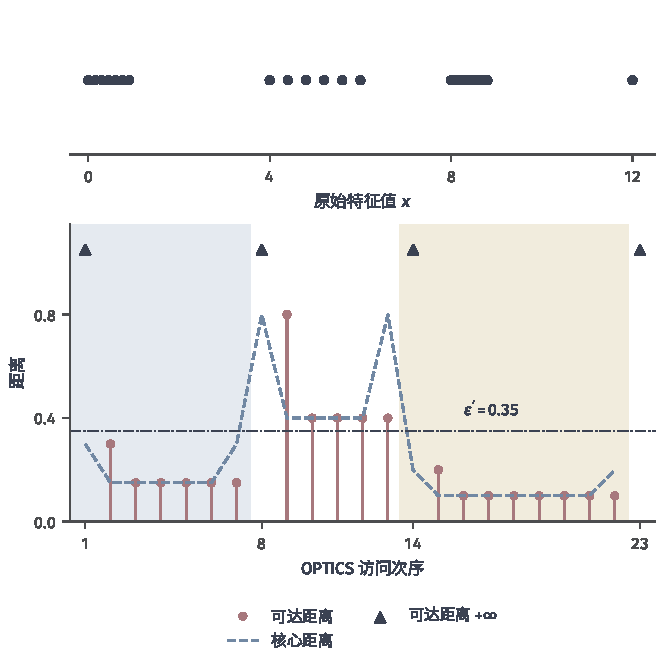
\includegraphics[width=105.412mm]{figures/04-classic-models/00-shared/matplotlib/clustering-optics-reachability/figure.pdf}
  \caption{固定一维教学数据上的OPTICS排序，取$\mathrm{MinPts}=3$（含自身）、$\varepsilon_{\max}=1.1$。三组样本的间距分别为$0.15$、$0.4$、$0.1$，另有$x=12$的孤立点。红色竖棒为可达距离，蓝色虚线为核心距离；蓝、黄底色标出两个低谷。无穷可达距离用顶部三角形表示，不能按其显示高度作数值比较；水平点划线展示阈值切割在本例中提取哪些低谷。}
 \label{fig:clustering-optics-reachability}
\end{figure}

低谷也可按相对陡降、陡升的$\xi$规则提取，并结合最小簇规模、前驱关系及嵌套处理。原始OPTICS已讨论陡峭区域，后续工作进一步构造密度层次。这里的自动提取减少人工读图，尺度和粒度仍由提取参数控制。

\subsubsection{理论分析}

\paragraph{表达能力}
OPTICS增加的是可供提取的密度尺度。对任意$\varepsilon'\leq\varepsilon_{\max}$，同时读取核心距离与可达距离，可以获得该尺度下的核心连通结构；若目标簇在某个这样的尺度满足前述DBSCAN邻接条件，它就在这份记录的可提取范围内。搜索上限之外的连接不会被记录，固定$m$下始终缺少邻居的小群体也不会因此变成核心簇。采用同一水平阈值提取时，疏密冲突依然存在；采用不同低谷的相对变化提取时，候选范围有所改变，但所需群组必须在相应低谷与边界中留下可区分的结构。记录多个尺度没有增加样本中缺失的分隔信息。



\paragraph{收敛性}
每个样本恰好进入输出次序一次，处理完$n$个样本后排序结束。若直接计算全部距离，邻域查询需要$O(n^2)$次距离计算；用二叉堆更新优先级，最坏可有$O(n^2)$次更新，每次代价$O(\log n)$。空间索引能减少一些数据上的搜索，但不改变高维或稠密邻域中的最坏情况。这里求解的是规定的访问次序及提取规则，不是迭代逼近某个全局最小损失。

\paragraph{泛化性}
\begin{theorem}[OPTICS预定有限尺度下的期望核心判定风险界]
对抽样前固定的$J$个半径及各自固定的质量阈值，若每个尺度的总体邻域质量与其阈值都相隔至少$\gamma>0$，可逐尺度应用定理\ref{thm:clustering-dbscan-core-risk}。令损失表示独立新点是否在至少一个尺度被误判为核心点，则并集界给出
\[
 \mathbb E_{D_n}R_{\mathrm{core}}\leq
       \min\{1,2J e^{-2n\gamma^2}\}.
\]
\end{theorem}

因此有限组预定尺度的核心判定可以同时推广到新点。可达图低谷的选择、簇标签的对应以及数据依赖的半径，仍需另行控制；这一结论不等于整条OPTICS层次的语义划分保证。

\subsubsection{优化表达能力}

OPTICS保存多个尺度的连接后，如何从这些尺度中选择群组仍需要规则。同一个尺度选择问题也可以用密度层次处理。Campello、Moulavi与Sander在2013年提出HDBSCAN框架，考察一个群组在多大尺度范围内持续存在，再据此提取簇\scite{clust-campello2013}。它另行构造层次，并非直接对OPTICS排序增加一个阈值。为了减小稀疏位置在较小尺度上过早连接的影响，它把两端点的核心距离$a_i,a_j$与原距离一起用于定义\term{互可达距离}（mutual reachability distance）：
\[
 \delta_{\mathrm{mr}}(i,j)
 =\max\{a_i,a_j,\delta(\bm{x}_i,\bm{x}_j)\}.
\]
在这一距离上构造最小生成树并形成密度层次，再按最小簇规模压缩层次、按跨尺度持续性选择簇，可以减轻单一$\varepsilon$的限制。代价是需要保存和处理层次，并明确最小簇规模及选择规则。

HDBSCAN的跨尺度持续性是层次中的簇选择量，评估抽样扰动还需要另外的统计协议。最小簇规模等参数继续控制输出，高维距离的区分度也需检验。密度路线将低密度分隔纳入簇定义；已有可信样本关系时，还可直接用图建立群组。

互可达距离使稀疏桥上的大核心距离成为连接下界，因而桥不会仅凭两点位置相近就在较小尺度接通。若目标群组分别在不同尺度形成并持续存在，它们可以出现在同一密度层次的不同分支中，随后由簇选择规则保留。若两个目标群组在所有保留尺度都没有分开，或目标小群体达不到最小簇规模，层次与持续性评分也不能创造这两个群组。最终选出的簇仍服从层次的包含关系，不能同时保留彼此交叉的两套分组。

\subsubsection{小结}

OPTICS把邻域搜索与划分提取分开，适合需要反复查看密度尺度的探索。它减少了更换阈值时的重复搜索，却增加了排序、优先队列和距离记录；$\varepsilon_{\max}$、$\mathrm{MinPts}$及提取规则继续决定哪些群组可以被读出。

HDBSCAN沿密度层次选择跨尺度持续的分支，回应的是怎样同时保留不同尺度的群组。它省去单一切割半径，仍需规定最小簇规模并承担层次构造成本。两种路线都要检查稀疏桥、小群体和高维距离，不能由多尺度记录本身推断语义分组已经正确。

\subsection{Mean Shift}
\label{sec:clustering-mean-shift}

密集路径与密度峰回答的是不同问题。两个聚集区域之间若有一条足够密集的连接带，DBSCAN可以把它们连为一簇；若希望把两处聚集峰分别识别出来，就需要考察密度在哪里达到局部高点。\term{均值漂移}（Mean Shift）先平滑估计密度，再把搜索点移向邻域样本的加权均值。在相应核条件下，这个移动方向与密度上升方向一致；从不同起点沿轨迹到达同一峰附近的样本可据此分组。平滑尺度会改变峰的数量，因此它也改变了所寻找的群组。

% 让历史段落自然接排，避免按整组引文高度提前截断正文。
Fukunaga与Hostetler在1975年从密度梯度估计出发，将局部均值偏移用于模式识别\scite{clust-fukunaga1975}。搜索先回答密度增加的方向，再据轨迹确定归宿，因此无需预先给出簇边界。

Cheng在1995年推广核与权重，讨论均值漂移、模态搜索和聚类之间的联系\scite{clust-cheng1995}。Comaniciu与Meer在2002年系统分析该方法，并展示特征空间和图像分割中的应用\scite{clust-comaniciu2002}。这些工作将密度上的移动规则与随后得到的簇分配联系起来，二者仍需分别规定停止与合并方式。

\subsubsection{模型结构}

以径向核估计未知密度。设 $h>0$ 为带宽，核函数为 $\mathcal{K}(\bm{u})=c_k k(\lVert\bm{u}\rVert_2^2)$，其中$c_k$是归一化常数，$k$是剖面函数（profile），规定核权重怎样随距离平方变化。则\term{核密度估计}（kernel density estimation, KDE）为
\begin{equation}
 \hat f(\bm{y})=\frac{c_k}{nh^d}
 \sum_{i=1}^n
 k\left(\frac{\lVert\bm{y}-\bm{x}_i\rVert_2^2}{h^2}\right).
 \label{eq:clustering-kde}
\end{equation}
可以从各样本出发在估计密度上搜索，把趋向同一模态的起点归为一簇。带宽决定平滑尺度，小带宽通常保留细节，大带宽通常合并邻近结构；模态数量的具体变化还依赖维数、核与样本分布。

\subsubsection{参数学习}

令 $g(u)=-k'(u)$，并记 $u_i(\bm{y})=\lVert\bm{y}-\bm{x}_i\rVert_2^2/h^2$。直接对式~\eqref{eq:clustering-kde} 求导可得
\[
 \nabla\hat f(\bm{y})=
 \frac{2c_k}{nh^{d+2}}
 \sum_i g(u_i(\bm{y}))(\bm{x}_i-\bm{y}).
\]
只要权重和为正，梯度便是正系数乘以\term{均值漂移向量}
\[
 \bm{m}(\bm{y})=
 \frac{\sum_i g(u_i(\bm{y}))\bm{x}_i}
      {\sum_i g(u_i(\bm{y}))}-\bm{y}.
\]
因此采用下列自适应步长的梯度方向更新：
\begin{equation}
 \bm{y}^{(t+1)}=
 \frac{\sum_i w_i^{(t)}\bm{x}_i}{\sum_i w_i^{(t)}},
 \qquad w_i^{(t)}=g(u_i(\bm{y}^{(t)})).
 \label{eq:clustering-mean-shift}
\end{equation}
权重来自一元剖面函数的负导数$g$，其自变量是距离平方。高斯剖面$k(u)=\exp(-u/2)$给出与高斯权重成比例的$g$，Epanechnikov剖面$(1-u)_+$在支撑内部给出常数权重，边界按分段规则处理。

式~\eqref{eq:clustering-mean-shift}与第\ref{sec:regression-nadaraya-watson}节的Nadaraya--Watson回归都计算核加权平均。Mean Shift平均输入位置，更新搜索点；核回归平均响应，预测条件均值。相同的平均运算承担不同的估计任务。

图~\ref{fig:clustering-mean-shift-modes}固定同一组一维样本，两个起点沿式~\eqref{eq:clustering-mean-shift}分别向左右峰移动，靠近驻点时位移减小。灰线改用更大带宽，两个峰合为一个峰。起点决定从哪里搜索，带宽改变估计密度及可到达的模态，两项选择因而影响不同的对象。

\begin{figure}[htbp]
  \centering
  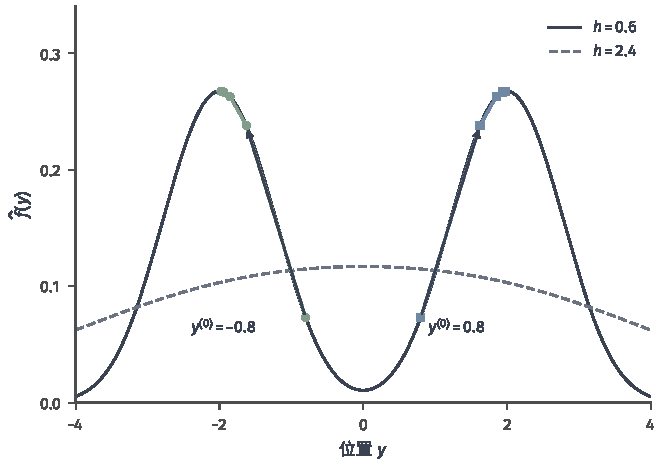
\includegraphics[width=105.412mm]{figures/04-classic-models/00-shared/matplotlib/clustering-mean-shift-modes/figure.pdf}
  \caption{Mean Shift 的密度爬升与带宽效应。左右各有三个样本，位置为 $-2.5,-2,-1.5$ 和 $1.5,2,2.5$，均采用高斯核。彩色标记给出带宽 $h=0.6$ 时从 $\pm0.8$ 出发的初始位置和四次更新，箭头指示第一次移动；灰色虚线对应 $h=2.4$，轨迹在黑色实线上计算。}
 \label{fig:clustering-mean-shift-modes}
\end{figure}

\begin{codeblock}[language=Python,label={code:clustering-mean-shift}]{高斯 Mean Shift 的起点更新}
import numpy as np

def mean_shift_positions(X, h, max_iter=300, tol=1e-4):
    X = np.asarray(X, dtype=float)
    if h <= 0:
        raise ValueError("h must be positive")
    Y = X.copy()
    for _ in range(max_iter):
        d2 = ((Y[:, None] - X[None]) ** 2).sum(2)
        log_w = -d2 / (2 * h * h)
        log_w -= log_w.max(1, keepdims=True)
        W = np.exp(log_w)
        new = (W @ X) / W.sum(1, keepdims=True)
        step = np.linalg.norm(new - Y, axis=1).max()
        Y = new
        if step <= tol:
            break
    return Y
\end{codeblock}

代码返回最终位置。得到簇标签还需合并相近终点，例如构造距离不超过$\rho$的终点图并取连通分量；$\rho=h/2$可作教学起点。这个合并阈值与更新容差用途不同，连通规则可能沿一串近终点把不同模态接在一起，需单独检查。

全部$n$个起点的一轮精确更新约需$O(n^2d)$运算。高斯核覆盖所有样本，因此截断邻域或近似近邻改变了精确更新。大数据实现可分块、减少起点或改用有限支撑核，并分别核对计算节省与位置误差。

\subsubsection{理论分析}

\paragraph{表达能力}
Mean Shift所拟合的是核平滑后的密度，输出则由其峰及吸引域确定。带宽对目标分组的影响可以用两个一维观测$-a,a$准确说明，其中$a>0$。取高斯核，两观测产生的密度与
\[
 e^{-(y-a)^2/(2h^2)}+e^{-(y+a)^2/(2h^2)}
\]
成比例，驻点满足$y=a\tanh(ay/h^2)$。在正半轴，右侧函数先以斜率$a^2/h^2$增长，随后斜率不断减小。若$a\leq h$，它不能再次越过直线$y$，唯一峰位于0；若$a>h$，两者在正半轴另有一个交点，负半轴对称地再有一个，0成为局部谷底，两侧各有一个峰。因而希望分别表示两处聚集时，过大的带宽会使两个峰在候选密度中消失，即使驻点求解完全准确也不能找回它们。

峰的吸引域也不等于密度连通簇。两个峰之间存在密集桥时，DBSCAN可以沿桥合并，Mean Shift仍可能按不同上升归宿分组；反过来，同一语义群体具有多个峰时，也可能被拆开。判断表达是否充分，需要先确认目标是平滑尺度下的模态分组，还是另一种关系；终点合并阈值还会进一步改变可保留的峰。

\paragraph{收敛性}
Mean Shift的上升不等式控制密度值，位置收敛还需排除轨迹在多个聚点之间移动。步长平方可和只说明步长趋零，后续研究指出了将它直接推为Cauchy性的缺口\scite{clust-aliyari2015}。下面用紧性、连续性和有限固定点补足这一步。

\begin{theorem}[Mean Shift在高斯核下的密度上升与条件收敛]
 \label{thm:clustering-mean-shift}
 设 $k$ 非负、凸、非增且可微，$k(0)<\infty$，迭代中权重和始终为正。则式~\eqref{eq:clustering-mean-shift} 产生的密度值单调不减且收敛。若进一步假设 $g=-k'$ 连续且严格为正，样本凸包内的固定点只有有限个，则位置序列也收敛，极限为 $\hat f$ 的驻点。
\end{theorem}
\begin{proof}
简记 $\bm{y}=\bm{y}^{(t)}$、$\bm{y}'=\bm{y}^{(t+1)}$。由凸性，
\[
 k(u_i(\bm{y}'))-k(u_i(\bm{y}))
 \geq g(u_i(\bm{y}))
       \bigl(u_i(\bm{y})-u_i(\bm{y}')\bigr).
\]
令 $w_i=g(u_i(\bm{y}))$、$s=\sum_iw_i$。由于 $\bm{y}'$ 是加权均值，展开平方后交叉项为零，得到
\[
 \sum_iw_i\bigl(
 \lVert\bm{y}-\bm{x}_i\rVert_2^2
 -\lVert\bm{y}'-\bm{x}_i\rVert_2^2\bigr)
 =s\lVert\bm{y}'-\bm{y}\rVert_2^2.
\]
所以
\begin{equation}
 \hat f(\bm{y}')-\hat f(\bm{y})
 \geq\frac{c_k s}{nh^{d+2}}
       \lVert\bm{y}'-\bm{y}\rVert_2^2\geq0.
 \label{eq:clustering-mean-shift-ascent}
\end{equation}
又有 $\hat f(\bm{y})\leq c_k k(0)/h^d$，故密度值收敛。

在附加条件下，第一次更新后所有位置均在有限样本的紧凸包内。距离平方因此有界，而连续正函数 $g$ 在相应紧区间上有正下界，故 $s$ 也有统一正下界。对式~\eqref{eq:clustering-mean-shift-ascent} 求和，得到步长平方可和，特别地，$\lVert\bm{y}^{(t+1)}-\bm{y}^{(t)}\rVert_2\to0$。

记连续更新映射为 $T$。任取收敛子列 $\bm{y}^{(t_j)}\to\bm{y}^\ast$，步长趋零与连续性给出 $T(\bm{y}^\ast)=\bm{y}^\ast$，所以每个聚点都是固定点。固定点有限，取彼此不相交的小球包围它们；序列最终必在这些小球的并集中，否则紧性会产生球外聚点。步长最终小于球之间的间隙，故序列不能再从一个球跳到另一个球。任意缩小球半径，便知它只能趋向其中一个固定点。梯度公式最后给出 $\nabla\hat f(\bm{y}^\ast)=\bm{0}$。
\end{proof}

位置收敛由紧性、连续性及有限固定点共同支持，平方可和用于先证明步长趋零。极限是驻点，特殊起点可能停在鞍点；解释为密度峰还需检查局部形状。Epanechnikov核的分段边界和零权重不满足第二部分的全部条件，需另作分析。

\paragraph{泛化性}
Mean Shift搜索的是训练样本构成的密度$\widehat f_h$。要判断这一对象是否接近总体，先评价密度估计误差，再考虑峰与吸引域；搜索当前密度的上升性不控制这项统计误差。

\begin{theorem}[Mean Shift所用KDE在二阶光滑密度下的期望估计误差]
 \label{thm:clustering-kde-risk}
设独立同分布观测的密度$f$定义在$\mathbb R^d$上，$f$二阶连续可微且平方可积，并满足
$\int\lVert\nabla^2f(\bm x)\rVert_F^2\,\mathrm d\bm x\leq A^2$。取非负积分为一的核$\psi$，满足
\[
 \begin{gathered}
 \int\bm u\psi(\bm u)\,\mathrm d\bm u=\bm0,\\
 m_2=\int\lVert\bm u\rVert_2^2\psi(\bm u)\,\mathrm d\bm u<\infty,
 \qquad\lVert\psi\rVert_{L^2}<\infty.
 \end{gathered}
\]
对带宽$h>0$的KDE
\[
 \widehat f_h(\bm x)=(nh^d)^{-1}\sum_i\psi((\bm x-\bm X_i)/h),
\]
有
\begin{equation}
 \mathbb E_{D_n}\lVert\widehat f_h-f\rVert_{L^2}^2
 \leq\frac{A^2m_2^2h^4}{4}
      +\frac{\lVert\psi\rVert_{L^2}^2}{nh^d}.
 \label{eq:clustering-kde-risk}
\end{equation}
\end{theorem}

证明将误差分成平方偏差与积分方差。二阶Taylor余项及核的一阶矩为零给出
$\lVert\mathbb E\widehat f_h-f\rVert_{L^2}\leq Am_2h^2/2$；独立样本使积分方差至多为$\lVert\psi\rVert_{L^2}^2/(nh^d)$。取$h$与$n^{-1/(d+4)}$同阶，两项合为$O(n^{-4/(d+4)})$。这是训练抽样平均的密度估计风险，适用于使用同一KDE的Mean Shift与DENCLUE。

该风险趋零仍未给出峰位置或新点簇标签的误差界。很平的峰可能随很小的密度扰动移动，吸引域边界附近的新点也可能改换归宿；从密度风险推进到这两个任务，需要控制导数误差、峰的曲率和边界附近的概率质量。带宽选择应对应所评价的任务。

\subsubsection{支持低密度背景排除场景}

Mean Shift按搜索归宿分组时，还需决定如何对待密度很低的驻点。沿同一平滑密度思路，Hinneburg与Keim在1998年提出DENCLUE，把各样本的影响函数相加，以密度阈值排除弱峰，再用吸引点及其连通关系组织簇\scite{clust-hinneburg1998}。网格减少密度计算需要访问的对象，同时要控制省略远处贡献的近似。它另行规定密度搜索、峰的保留与计算组织，高维估计是否可靠仍取决于样本量、表示和核尺度。

若任务把低于$t$的密度区域视为背景，DENCLUE的阈值允许这部分对象不形成独立簇，比基本Mean Shift保留所有模态更接近该目标。它所保留的区域仍属于指定影响函数产生的平滑密度：两个目标群组之间若在这一密度的$t$水平以上连通，按密度连接合并时就不能把它们分开；一个目标群组的最高密度若低于$t$，则会被整体排除。降低$t$可以保留弱群组，也可能把背景连接一并纳入。

\subsubsection{小结}

Mean Shift适合寻找平滑密度中的聚集峰，以局部加权均值推进搜索，再按归宿组织样本。簇数取决于带宽、起点和终点合并；图像分割与跟踪可以利用这种聚集机制，但弱峰、平坦驻点和反复邻域访问都需要处理。

若背景中的弱峰不应独立成簇，DENCLUE用阈值规定保留哪些吸引点，并允许根据密度连接合并它们。阈值会同时改变弱群体与背景的取舍，网格近似则改变密度计算预算。这条路线与基本模态归宿分组的区别在簇提取规则，不能仅根据两者都使用密度爬升就认为输出相同。

\subsection{模型对比与总结}

密度方法有两种不同的群组定义。DBSCAN把满足计数条件的核心点沿邻域连接，再接纳边界点；同一条弯曲的密集路径可以成为一簇，低密度对象则作为噪声。Mean Shift先估计平滑密度，把到达同一峰的搜索轨迹归为一组。两处密度峰之间即使有足够密集的连接带，也可能在DBSCAN中合为一簇、在Mean Shift中分成两组。前者保留连通区域，后者区分聚集归宿，选择首先取决于要解释哪一种结构。

在连通路线中，DBSCAN的单一半径难以同时照顾稠密簇和稀疏簇：照顾稀疏簇所需的大半径也可能接通稠密簇之间的桥。OPTICS保存可达排序及距离，把邻域搜索与尺度提取分开，便于观察哪些群组在不同尺度出现；它仍需提取规则，使用同一水平阈值时也仍会遇到疏密冲突。HDBSCAN另建互可达距离的层次，再根据最小簇规模及跨尺度持续性选分支，使不同群组可以在不同密度尺度上保留。它与OPTICS共享对多尺度结构的关注，层次构造和选择准则则不同。

在模态路线中，带宽决定Mean Shift看到的是许多细峰还是少数宽峰。若低密度背景中的弱峰不应独立成簇，DENCLUE通过密度阈值筛选吸引点，并按密度连接组织群组；它同时改变了峰的保留和合并方式。阈值降低会保留更多弱群体，也可能纳入背景连接，因而不能只把它看成更快的Mean Shift。

这些调整分别回应单一尺度、弱峰和连接规则的问题，没有消除表示与距离选择的责任。比较时应检查目标小群体是否被保留、桥接是否符合用途，以及查询、密度估计和层次提取的成本；同一二维散点图上的相近划分，可能来自不同的簇定义。

\section{基于图的聚类}
\label{sec:clustering-graph}

社交连接、文档相似度和像素邻接可以直接表示为加权图。图聚类将样本作为顶点、相似程度作为边权，寻找内部连接较强而外部连接较弱的群组。向量距离也可用于建图；边权和邻域规则因此继续决定所保留的相似关系。

仅最小化切边权重，可能轻易切下一个连接少的小块。对簇规模或连接体积作归一化，可以比较“割断多少联系”与“簇原来拥有多少联系”。谱聚类再把这一离散搜索松弛为特征向量求解。

\subsection{谱聚类}
\label{sec:clustering-spectral}

弯曲点带还可以用图来表示：只给相近样本连边，同一条带内有许多连接，两条带之间只有很少连接。分组便转为切断较少的跨组联系。不过，直接寻找最优图划分需要搜索组合众多的标签方案。\term{谱聚类}（spectral clustering）先将离散标签放松为连续数值，用图拉普拉斯的特征向量求取低成本的连续表示，再在该表示上划分顶点。它改变了中心方法所使用的坐标，但分组结果仍取决于图是否保留了可信的相似关系。von Luxburg的教程整理了图构造、归一化及适用条件\scite{clust-luxburg2007}。

第\ref{sec:dim-le}节的拉普拉斯特征映射共享建图与低频谱表示，直接输出连续坐标；谱聚类还需要离散分配。下面以归一化割及多簇谱算法说明这两步怎样衔接。

Donath与Hoffman在1973年用谱信息给图划分代价建立下界，将组合搜索与可计算特征值联系起来\scite{clust-donath1973}。Shi与Malik进一步用像素相似关系建立归一化割，相关会议和期刊论文分别发表于1997年和2000年\scite{clust-shi2000}。Ng、Jordan与Weiss在2001年会议提出多簇谱嵌入与行归一化，论文集于2002年出版\scite{clust-ng2002}。这些工作分别解释了图目标、连续表示及离散化的连接。

\subsubsection{模型结构}

设无向图的非负对称权重矩阵为 $\bm{W}\in\mathbb{R}^{n\times n}$，通常令 $w_{i,i}=0$。向量样本可用高斯相似度 $\exp(-\lVert\bm{x}_i-\bm{x}_j\rVert_2^2/(2\sigma^2))$ 构造边；近邻图则保留部分局部关系。单向近邻关系未必对称，必须明确采用并集对称化还是互近邻规则。

定义顶点度 $d_i=\sum_jw_{i,j}$、度矩阵 $\bm{D}=\operatorname{diag}(d_1,\ldots,d_n)$，以及三种拉普拉斯：
\begin{align}
 \bm{L}&=\bm{D}-\bm{W},\nonumber\\
 \bm{L}_{\mathrm{sym}}
 &=\bm{I}-\bm{D}^{-1/2}\bm{W}\bm{D}^{-1/2},\nonumber\\
 \bm{L}_{\mathrm{rw}}
 &=\bm{I}-\bm{D}^{-1}\bm{W}.
 \label{eq:clustering-laplacians}
\end{align}
归一化所用逆度数要求$d_i>0$，因此先单独处理孤立顶点。$\bm{L}_{\mathrm{rw}}$ 一般不对称，但与 $\bm{L}_{\mathrm{sym}}$ 相似，因而有相同的实特征值。对任意 $\bm{v}\in\mathbb{R}^n$，
\begin{equation}
 \bm{v}^{\top}\bm{L}\bm{v}
 =\frac12\sum_{i,j}w_{i,j}(v_i-v_j)^2\geq0.
 \label{eq:clustering-laplacian-form}
\end{equation}
所以 $\bm{L}$ 半正定，且 $\bm{L}\bm{1}=\bm{0}$；零特征值的重数等于连通分量数，图连通时才为单重。

归一化还具有随机游走解释。转移矩阵 $\bm{P}=\bm{D}^{-1}\bm{W}$ 让游走者按边权比例选择下一顶点，且 $\bm{L}_{\mathrm{rw}}=\bm{I}-\bm{P}$。从一个簇出发，若内部连接强而外部连接弱，游走就倾向在簇中停留较久；Meilă 与 Shi 据此研究了聚类的随机游走视角\scite{clust-meila2001}。

设 $\operatorname{cut}(A,\bar A)=\sum_{i\in A,j\notin A}w_{i,j}$，$\operatorname{vol}(A)=\sum_{i\in A}d_i$。\term{归一化割}（normalized cut, NCut）定义为
\begin{equation}
 \operatorname{NCut}(\mathcal{P})
 =\sum_{k=1}^K
 \frac{\operatorname{cut}(C_k,\bar C_k)}
      {\operatorname{vol}(C_k)}.
 \label{eq:clustering-ncut}
\end{equation}
它比较切边与簇内外连接体积，减轻小簇的偏好；同体积的簇可以含不同样本数\scite{clust-shi2000}。\term{比率割}（RatioCut）则把分母换成 $|C_k|$，对应未归一化拉普拉斯的松弛。

\subsubsection{参数学习}

为把 NCut 改写成矩阵目标，定义 $\bm{F}\in\mathbb{R}^{n\times K}$，其中
\[
 f_{i,k}=
 \begin{cases}
  1/\sqrt{\operatorname{vol}(C_k)},&i\in C_k,\\
  0,&i\notin C_k.
 \end{cases}
\]
簇互不相交给出 $\bm{F}^{\top}\bm{D}\bm{F}=\bm{I}_K$。由式~\eqref{eq:clustering-laplacian-form}，第 $k$ 列的二次型恰为第 $k$ 项归一化割，故目标为 $\operatorname{tr}(\bm{F}^{\top}\bm{L}\bm{F})$。

困难在于每行只允许一个特定的非零值。去掉这一离散约束，令 $\bm{H}=\bm{D}^{1/2}\bm{F}$，得到
\begin{equation}
 \min_{\bm{H}^{\top}\bm{H}=\bm{I}_K}
 \operatorname{tr}(\bm{H}^{\top}
                   \bm{L}_{\mathrm{sym}}\bm{H}).
 \label{eq:clustering-spectral-relaxation}
\end{equation}
Shi--Malik 方法也可写为广义特征问题 $\bm{L}\bm{f}=\lambda\bm{D}\bm{f}$，与归一化变换相联系\scite{clust-shi2000}。取 $\bm{L}_{\mathrm{sym}}$ 最小的 $K$ 个特征值对应的特征向量，即得到式~\eqref{eq:clustering-spectral-relaxation} 的最优解；下文说明这一连续最优值及其唯一性条件。

连续解还需离散化。\term{NJW 算法}把 $\bm{H}$ 每一行归一化到单位长度，再对行向量运行 K-means\scite{clust-ng2002}。若图恰有 $K$ 个连通分量，理想谱空间中每个分量对应同一方向；行归一化消除度数造成的长度差异，图~\ref{fig:clustering-spectral} 展示了这一解释。连接较弱的实际图中，这只是近似结构。

\Needspace{62mm}
\begin{figure}[htbp]
  \centering
  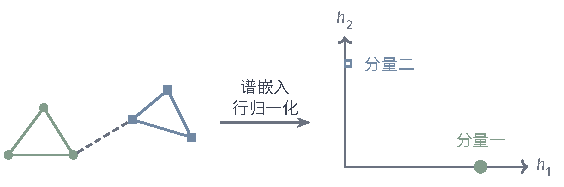
\includegraphics[width=95.564mm]{figures/04-classic-models/00-shared/tikz/clustering-spectral/figure.pdf}
  \caption{谱聚类的理想情形：圆形与方形分别标识两个互不连接的分量，颜色只作辅助；在归一化谱空间中，两个分量分别落到两个方向。细虚线表示实际数据中可能存在的弱连接；加入这些连接后，谱坐标通常形成近似群组。}
 \label{fig:clustering-spectral}
\end{figure}

\begin{codeblock}[language=Python,label={code:clustering-spectral}]{给定相似度矩阵的 NJW 算法}
import numpy as np
from scipy.linalg import eigh

def spectral_clustering(W, K):
    W = np.asarray(W, dtype=float)
    n = len(W)
    if W.shape != (n, n) or not 1 <= K <= n:
        raise ValueError("invalid shape or K")
    if (W < 0).any() or not np.allclose(W, W.T):
        raise ValueError("W must be nonnegative and symmetric")
    degree = W.sum(1)
    if (degree <= 0).any():
        raise ValueError("handle isolated vertices first")
    inv = 1 / np.sqrt(degree)
    L = np.eye(n) - inv[:, None] * W * inv[None, :]
    _, H = eigh(L, subset_by_index=[0, K - 1])
    length = np.linalg.norm(H, axis=1)
    if (length == 0).any():
        raise ValueError("zero embedding row")
    labels, _ = kmeans(H / length[:, None], K)
    return labels
\end{codeblock}

代码复用代码~\ref{code:clustering-kmeans}的K-means函数，处理能放入内存的稠密矩阵。图的连通分量数超过$K$时，所选零特征子空间可能含零行，也可能将多个分量任意合并。应先确定各连通分量是否需要独立输出，再选择谱子空间与分配策略。

稠密建图约需$O(n^2d)$距离运算和$O(n^2)$存储，完整特征分解约需$O(n^3)$。只求部分特征向量时，可用Lanczos或LOBPCG，矩阵乘法成本可按稀疏边数计算；迭代总成本还受特征间隙、精度和迭代次数影响。大规模实现可结合近邻图或Nyström近似，并核对它们对谱表示的误差。

\subsubsection{理论分析}

\paragraph{表达能力}
离散NCut的候选是图顶点的$K$簇划分，并不要求每簇在原向量空间中凸。对两条没有跨带边、各自内部连通的弯曲点带，取$K=2$，按点带划分的NCut为零，已达到非负目标的最小值。这比原空间两个Voronoi单元更能表达“一条带一簇”。

有跨组边时，目标划分仍在离散候选中，但不一定是NCut最优。若两个语义群组之间有很强连接，而另一个较小切口的相对边权更低，图割就会偏向后者。谱方法对非凸形状的收益因此来自可信的局部连接，而非低维谱坐标无条件地恢复了语义类别。

\paragraph{收敛性}
谱聚类的求解分为特征子空间计算与离散分组。前一阶段要找到最小的$K$个特征值及其子空间，并达到残差精度；后一阶段的K-means另有初始化与停止条件。下面先确定连续松弛的全局最优值，随后再说明它与离散图割质量的关系。

在式~\eqref{eq:clustering-spectral-relaxation}中，令$\bm B=\bm L_{\mathrm{sym}}$，并取$1\leq K\leq n$。将这个实对称谱算子的特征值按升序记为$\lambda_1\leq\cdots\leq\lambda_n$，对应标准正交特征向量为$\bm u_1,\ldots,\bm u_n$。正交列约束下的连续松弛最优值为
\[
 \min_{\bm H^\top\bm H=\bm I_K}
 \operatorname{tr}(\bm H^\top\bm B\bm H)
 =\sum_{k=1}^K\lambda_k.
\]
取$\bm H=[\bm u_1,\ldots,\bm u_K]$即可达到该值。若$K<n$且$\lambda_K<\lambda_{K+1}$，最优列空间唯一，但其中的正交基仍可右乘正交矩阵（参考\BookTheoremRef{thm:matrix-analysis-trace-minimum}{卷1《数学准备：计算、分析与几何》第5章“线性空间”第5.5.4节“秩约束下的矩阵逼近”}）。这个结论确定的是连续子空间；把它转换成离散簇标签，还需要前述离散化步骤。

在理想图上，谱松弛与离散化可以保留原图割目标：若图恰有$K$个连通分量且所有顶点度为正，零特征空间由各分量的度加权指示向量张成。行归一化后，同一分量的行完全相同，不同分量的行对应不同正交方向，因而全局最优的$K$-means离散化可给出零失真并恢复这$K$个分量。

即使特征向量计算准确，也只说明得到了该图的连续最优解；错误边权改变了目标，松弛和离散化还可能留下额外差异。

图割质量与谱量之间还存在 Cheeger 型联系。对连通、非负无向图，定义\term{电导}（conductance）
\[
 \phi(S)=
 \frac{\operatorname{cut}(S,\bar S)}
 {\min\{\operatorname{vol}(S),\operatorname{vol}(\bar S)\}},
 \qquad h_G=\min_{\varnothing\ne S\ne V}\phi(S).
\]
若 $\lambda_2$ 是 $\bm{L}_{\mathrm{sym}}$ 的第二小特征值，则
\begin{equation}
 \frac{\lambda_2}{2}\leq h_G\leq\sqrt{2\lambda_2}.
 \label{eq:clustering-cheeger}
\end{equation}
图上的这类不等式把低频特征向量与稀疏切割联系起来，标准谱图论教材给出了证明及其与流形版本的关系\scite{clust-chung1997}。

这里$h_G$最小化电导，NCut则对两个方向分别按体积归一；二者的关系需由分母比较得到。二分情形满足 $\phi(S)\leq\operatorname{NCut}(S,\bar S)\leq2\phi(S)$。若 $\bm{u}$ 是 $\bm{L}_{\mathrm{sym}}$ 的第二特征向量，则
\[
 \bm{f}=\bm{D}^{-1/2}\bm{u},
 \qquad
 \bm{L}\bm{f}=\lambda_2\bm{D}\bm{f},
 \qquad
 \bm{L}_{\mathrm{rw}}\bm{f}=\lambda_2\bm{f}.
\]
因此，Cheeger sweep 应按 $f_i=u_i/\sqrt{d_i}$ 排序并扫描阈值；若直接求广义特征问题或随机游走拉普拉斯，排序坐标就是其特征向量 $\bm{f}$。只有各顶点度数相同时，按 $\bm{u}$ 与按 $\bm{f}$ 排序才必然相同。这一保证对应二分的阈值扫描；多簇NJW加K-means使用另一离散化规则，其图割质量需另行分析。

\paragraph{泛化性}
谱聚类的训练输出是给定图的划分，先前的Cheeger界可以解释成该图上的关系损失。设图连通、权重对称非负，$S$为非空真子集，$I$在$S$内按$d_i/\operatorname{vol}(S)$抽取，再按$w_{ij}/d_i$走一步到$J$。离开$S$的概率为
\[
 P(J\notin S\mid I\in S)
 =\frac{\operatorname{cut}(S,\bar S)}{\operatorname{vol}(S)}.
\]
从$\bar S$开始的离开概率同理；二者之和恰为$\operatorname{NCut}(S,\bar S)$。按第二特征向量的正确归一化坐标作阈值扫描，Cheeger结论保证存在输出$\widehat S$使
\begin{equation}
 R_G(\widehat S):=\operatorname{NCut}(\widehat S,\bar{\widehat S})
 \leq2\sqrt{2\lambda_2}.
 \label{eq:clustering-spectral-graph-risk}
\end{equation}
这是冻结图后，对图上随机游走的期望跨簇损失；它没有对新的独立对象给出风险界。多簇NJW加K-means也不能直接套用这个二分扫描结论。

总体分布上的评价还需指定建图制度与新点分配。固定相似核时，经验谱对象可以向总体积分算子收敛\scite{clust-luxburg2008}，但算子或子空间一致性尚未给出新点分组损失，离散化、簇匹配和边界处的概率质量仍需控制。带宽随$n$改变的流形极限则有另一组采样、带宽及归一化条件。本节的明确风险保证止于式\eqref{eq:clustering-spectral-graph-risk}所规定的有限图任务。

\subsubsection{支持样本对关系监督场景}

如果已知某两条记录应当同簇，或另一对记录应当异簇，就可以让这些关系改变谱聚类所用的图。Kamvar、Klein与Manning的Spectral Learning研究了将监督信息纳入谱表示；一种直接做法是提高应同簇样本对的边权、降低应异簇样本对的边权，再对修改后的非负对称图求谱表示\scite{clust-kamvar2003}。

边权调整改变谱偏好，最终分配仍由整张图和离散化决定。即使删除应异簇样本对之间的边，两端也可能通过其他强边共簇。修改后的非负对称图可按其新拉普拉斯分析，但谱间隙、连接及统计条件需重新核对。关系传播还能扩展局部监督，同时可能扩散错误信号。

\subsubsection{小结}

谱聚类以关系图保留非凸连接结构，用特征分解求连续松弛，再通过离散化形成簇。图构造与最后分配共同影响结果。特征值间隙可作为探索$K$的线索，解释时还需排查噪声、弱连接与孤立分量造成的间隙。

\subsection{代表选择与消息传播}
\label{sec:clustering-affinity-propagation}

谱聚类希望划分连接较强的群组。如果任务更重视“每组由哪条记录代表”，就可以回到真实样本代表的思路。K-medoids需要预先指定代表数，Frey与Dueck在2007年提出的\term{近邻传播}（Affinity Propagation, AP）则让每个样本都成为潜在代表，通过两类消息协调选择。

\subsubsection{模型结构}

适合度描述样本对一个候选代表的支持，可用度汇总该候选能否作为代表的其他支持；对代表本身设置的偏好间接控制代表数。

\subsubsection{参数学习}

给定相似度$s(i,k)$，其典型更新为
\[
 r(i,k)=s(i,k)-\max_{k'\ne k}\{a(i,k')+s(i,k')\},
\]
\[
 a(i,k)=
 \min\left\{0,r(k,k)+
 \sum_{i'\notin\{i,k\}}\max\{0,r(i',k)\}\right\},
 \quad i\ne k,
\]
而 $a(k,k)=\sum_{i'\ne k}\max\{0,r(i',k)\}$。适合度衡量候选相对其他代表的优势，可用度汇总其他样本对该代表的支持。对角相似度 $s(k,k)$ 是偏好参数，间接控制代表数；通常还需阻尼以缓解振荡，迭代不保证总收敛\scite{clust-frey2007}。

消息更新后，以两类消息之和比较候选代表，并按预定平局规则选择代表索引
\[
 e_i\in\argmax_k\{a(i,k)+r(i,k)\}.
\]
同一代表对应同一簇，即$C_k=\{i:e_i=k\}$。输出要求代表选择连续若干轮稳定且相互一致：一个样本选择$k$时，$e_k=k$，即代表选自身。中间迭代可能尚未满足这两个条件，此时继续更新或返回未收敛状态，保留当前消息供诊断。

\subsubsection{理论分析}

\paragraph{表达能力}
AP的候选仍是由真实对象作代表的分组。若非对角相似度取负平方欧氏距离，固定所选代表后，其他对象按最大的相似度选择代表，沿用最近中心区域的限制；内外同心圆也不会仅因消息传递而变成两个可准确表示的簇。改变对角偏好允许更多或更少代表参与目标，能适应不同量化精度，却没有规定哪个代表数就是语义簇数。一般关系相似度可以表达不同分组，但必须在这些关系中提供目标所需的区别。



\paragraph{收敛性}
代表索引的候选数有限，所以相似度总和目标存在最优可行分组。但是消息并非在这个有限集合上作严格下降搜索，而是连续数值的迭代，可能振荡；阻尼不能无条件保证收敛。一次稠密更新可通过缓存各行最大值、次大值及各列正贡献和在$O(n^2)$时间内完成，消息存储同为$O(n^2)$。设置$T$轮上限只能给出$O(Tn^2)$的预算，最终还需检查代表自选与归属一致性。

\paragraph{泛化性}
\begin{theorem}[AP冻结欧氏代表在独立验证下的期望量化风险界]
当相似度采用负平方欧氏距离时，可以冻结训练选出的代表，并按最近代表分配新点。若输入范数至多为$r$，平方距离损失位于$[0,4r^2]$。条件于训练过程，用独立的$m$个同分布观测计算冻结规则的平均损失$\widehat R_m^{\mathrm{val}}$，Hoeffding界直接给出，以至少$1-\delta$的概率，
\[
 R\leq\widehat R_m^{\mathrm{val}}
       +4r^2\sqrt{\frac{\log(1/\delta)}{2m}}.
\]
\end{theorem}

这里无需预定代表数，但规则必须在读取验证样本前冻结。一般关系相似度未必能计算新对象与代表的关系，届时需要先补足新点分配和损失，不能直接套用平方距离结论。

\subsection{度数基准下的社区划分}

若图记录的是社交联系，高度活跃的顶点本来就会拥有很多边，仅凭簇内边多还不能说明形成了特殊群体。Louvain方法优化\term{模块度}（modularity），把实际簇内边权与保留顶点度数的随机基准比较，寻找内部连接超出该基准的社区。它不要求选出典型代表，也不同于直接最小化归一化割。

\subsubsection{模型结构}

令$2m_G=\sum_i d_i$，典型目标为
\[
 Q=\frac{1}{2m_G}\sum_{i,j}
 \left(w_{i,j}-\frac{d_i d_j}{2m_G}\right)
 \mathbb{1}\{c_i=c_j\}.
\]
\subsubsection{参数学习}

局部顶点移动提高模块度，社区凝聚再改变搜索规模，稀疏图可减少边访问。结果仍受分辨率、移动顺序和局部极值影响；其目标与NCut不同，保证应按模块度搜索核对\scite{clust-blondel2008}。

\subsubsection{理论分析}

\paragraph{表达能力}
模块度也没有把“连接少就应该分开”写成无条件规则。记$w(A,B)$为两个不同社区之间的总边权，$v_A,v_B$为它们的度数之和，由上式直接计算，合并两社区使模块度改变
\[
 \Delta Q=\frac{w(A,B)}{m_G}-\frac{v_Av_B}{2m_G^2}.
\]
只有跨社区边权超过该度数基准时，合并才提高模块度。这个判据依赖全图总边权$m_G$；其他区域的边权变化也可能改变这两个社区应否合并。任意顶点划分都可以作为候选，但目标偏好的是相对于全图基准的连接富集，不能把它直接等同于预定语义群组。Louvain的局部搜索另外限制了哪些候选能被实际找到。



\paragraph{收敛性}
固定有限顶点集时，划分数量有限，模块度最大值必然存在。若只接受严格增益的顶点移动，则一个阶段不能重复访问同一划分；凝聚后只要社区数严格减少，就至多进行$n-1$次这样的规模缩减。零增益移动须有禁止循环的规则。这些条件保证有限停止，不能保证找到所有划分中的最大模块度；分辨率和局部搜索的限制仍然保留。

\Needspace{8\baselineskip}
\paragraph{泛化性}
\begin{theorem}[Louvain冻结划分在独立同分布图上的期望模块度损失界]
当前图上的高模块度只评价当前边。若用途是同一组顶点在未来时段是否仍形成社区，可以把各时段的整张图作为观测：冻结训练图选出的划分$c$，假设验证图$G_1,\ldots,G_m$与未来图独立同分布、均具有非负无向边权且总度数为正。用$\ell_c(G)=1-Q_G(c)$评价社区在新图上相对度数基准的表现。由于$Q_G(c)\in[-1,1]$，损失在$[0,2]$内，故以至少$1-\delta$的概率，
\[
 \mathbb E_G[1-Q_G(c)]
 \leq\frac1m\sum_{j=1}^m[1-Q_{G_j}(c)]
        +2\sqrt{\frac{\log(1/\delta)}{2m}}.
\]
\end{theorem}

这是对未来整图的风险保证，抽样单位是图，不是同一张图中相互依赖的边；它也未定义新顶点加入后的归属。只有一张图时，不能把训练模块度代入此式充当独立验证。

\subsection{模型对比与总结}

图关系提供了共同输入，却没有规定唯一的分组目标。谱聚类希望切断较少的跨组联系，同时避免只切出连接很少的小块，因此使用归一化割等准则，再通过特征向量松弛减少离散搜索。它适合关系图中的连通群组，代价在构图、谱求解及最后离散化；通常仍需指定$K$，图中的错误桥接也会进入低维表示。

AP转向“哪条记录代表这一组”。它与K-medoids一样保留真实对象作为代表，通过消息协调代表选择，并用对角偏好代替显式指定代表数。消息搜索减少了直接枚举代表集合的需要，却引入偏好、阻尼和未收敛状态。它不是谱割目标的另一种求解器：负欧氏距离相似度仍偏好靠近同一代表的对象，消息传递本身不会增加环形群组的表达。

Louvain又针对关系网络中的度数差异。活跃顶点本来就会带来很多边，模块度因此把簇内联系与度数基准比较，再用局部移动和社区凝聚搜索划分。它省去预定$K$和特征分解，主要成本落在边访问与多层局部搜索；全图基准也带来分辨率问题，顶点移动顺序可能影响局部结果。高模块度社区未必具有最低归一化割，也未必由某个典型对象代表。

因此三种方法是围绕不同输出和目标形成的路线。需要低跨组连接时检查图割与构图，需要展示典型记录时检查代表及偏好，需要解释超出度数基准的联系时检查模块度与分辨率。比较它们应先确定共同用途，再衡量该用途下的分组和资源代价，不能把三个目标值直接排列为优劣。

\section{基于网格与子空间的聚类}
\label{sec:clustering-subspace}

大样本的点对访问可能超过预算，无关特征也可能掩盖只在少数坐标上聚集的群组。一些高维分布会使最近与最远距离的相对差异减小；是否发生这种集中，仍取决于数据结构与表示。网格和子空间方法分别处理重复访问与相关坐标选择。

网格方法把样本汇为单元统计，减少随后查询原始点的次数。子空间方法寻找群组在哪些坐标上紧凑，并允许各簇使用不同特征。CLIQUE结合两者，以计数剪枝降低候选搜索；已存单元和子空间组合也可能随维数快速增长，需要计入资源预算。

\subsection{STING}

对同一批地理位置记录，我们可能反复查询不同区域内有多少对象、哪些地方足够密集。如果每次都读取所有记录，许多统计会被重复计算。\term{统计信息网格}（STatistical INformation Grid, STING）把空间分成大小不同的层次单元，预先保存每个单元的计数、均值等统计，查询时先排除无关区域，再向需要细查的单元下钻。Wang、Yang与Muntz在1997年提出了这一方法\scite{clust-wang1997}。它主要改变数据访问方式，单元大小同时限定了直接从摘要读出的空间精度。

\subsubsection{模型结构}

STING通常用于低维空间的矩形层次网格。二维单元可分为四个子单元，$d$维完整二分则产生$2^d$个子单元。实现可只保存有记录或需要查询的单元，以控制空单元的存储。

单元摘要包含计数、各维均值、标准差、极值与分布类型估计。计数、和及平方和可由子单元相加，得到父单元的矩统计。分布类型则属于近似描述：子单元合并后形成混合，父单元可能超出原分布族。

\subsubsection{参数学习}

构建阶段扫描样本，确定最细单元并更新统计，再自底向上汇总。固定维数和网格规模时可按 $O(n)$ 扫描成本理解；更完整地计入维数与 $G$ 个已存单元，代价包含 $O(nd+Gd)$，还取决于定位单元的数据结构。

查询时，从某层网格出发，依据摘要估计单元满足条件的可能性。例如，对密度条件使用计数，对属性范围条件使用极值或分布近似；排除不相关单元，对保留单元继续下钻。最终可以把满足密度条件且相邻的单元连成区域，必要时回到原始样本作精确检查。

固定摘要上的单元访问约按$O(G)$计，初始读入与统计仍需前述样本扫描。精确查询若最终检查$n_{\mathrm{scan}}$条原始记录，也应另外计费。基于估计概率的排除可能漏检；需要完整结果时，筛选规则须能证明被排除区域无法满足查询。

\subsubsection{理论分析}

\paragraph{表达能力}
只用网格计数判定密集区域时，STING的候选是单元的并，最细单元内的位置差异没有进入这一判据。若两个目标群组落在同一个单元内，仅凭该单元的计数就不能把它们分开；若保留相邻密集单元形成一条路径，连接规则也会把路径两端合并。回到原始记录可以细分，但此时已经增加了摘要之外的信息。

对密度目标也可以量化这种限制。设总体密度$f$定义在$[0,1]^d$上，完整网格的边长为$h$，并满足Lipschitz条件$|f(\bm x)-f(\bm y)|\leq L\lVert\bm x-\bm y\rVert_2$。把每个单元上的密度用其平均值$f_h$表示，则
\[
 \lVert f_h-f\rVert_\infty\leq L\sqrt d\,h,
\]
因为单元直径为$\sqrt d\,h$。细化网格可以降低这份表示误差；固定网格时，即使单元质量已知，也保留了单元内变化的误差。摘要中的均值、方差和分布类型可以补充局部描述，却不能无条件确定一个单元内任意的多峰分布。



\paragraph{收敛性}
固定网格层次后，统计计数由有限次累加得到，不存在局部极值或迭代收敛问题。若层次深度为$H$，每个样本沿唯一的网格路径更新，直接统计需要$O(nH)$次网格访问；对共有$G$个格的已建层次作一次查询，最坏访问$O(G)$个格。若另外计算$d$维均值等统计量，还需相应的坐标运算。这里的精确性针对网格统计，不表示固定网格已经充分逼近任意密度边界。

\paragraph{泛化性}
STING的计数摘要可以估计总体区域质量，完整的细网格还可作直方图密度估计。

\begin{theorem}[STING在固定网格下的期望密度估计误差]
 \label{thm:clustering-sting-risk}
设独立同分布样本的密度$f$定义在$[0,1]^d$上，满足$|f(\bm x)-f(\bm y)|\leq L\lVert\bm x-\bm y\rVert_2$。预先固定边长$h$的等体积网格，$1/h$为整数，每个单元$U$上令
$\widehat f_h=n(U)/(nh^d)$。则
\begin{equation}
 \mathbb E_{D_n}\lVert\widehat f_h-f\rVert_{L^2}^2
 \leq L^2d h^2+\frac1{nh^d}.
 \label{eq:clustering-sting-risk}
\end{equation}
\end{theorem}

单元内密度与其平均值的差至多为$L\sqrt d\,h$，给出平方偏差项；单元计数的二项方差相加，给出$1/(nh^d)$的上界。这保证摘要构成的密度估计，未保证按密度阈值连接出的区域稳定；后者还需阈值间隔等条件。WaveCluster对计数再作小波变换，也需分别控制变换后的估计误差与区域提取，不能把平滑外观直接当作群组泛化保证。

\subsubsection{优化泛化能力}

细网格能够分开邻近群组，却也会留下细尺度计数波动。Sheikholeslami、Chatterjee与Zhang在1998年的WaveCluster中把网格计数作为离散信号，在不同小波尺度寻找密集区域，并抑制部分高频噪声\scite{clust-sheikholeslami1998}。它与STING共享网格摘要的输入方式，另外增加了变换与区域筛选，并不是保留原查询目标的计算加速。

分辨率继续限定边界精度；小波变换后的筛选又决定保留哪些空间变化。若两处聚集的分隔只体现于被舍弃的细尺度系数，平滑结果就可能把它们合在一起。保留较细尺度可以表达这个间隔，却也会保留相应尺度的计数波动。固定维数、网格及变换规模时，读入成本可随样本数线性增长，网格变换和区域提取仍需单独计入。

\subsubsection{小结}

STING把反复读取记录转为查询层次网格摘要，适合低维区域查询与增量统计。单元越细，边界信息越多，存储与下钻成本也越高；需要摘要未保存的关系时，仍须回查原始记录。

若任务转为在计数中寻找多尺度密集区域，WaveCluster再对网格信号作小波处理。它可以筛除部分细尺度波动，也可能舍弃区分邻近群组的细节。因此网格大小回答“保留多细的空间位置”，变换与筛选回答“保留哪些空间变化”，两者应分别选择。

\subsection{CLIQUE}
\label{sec:clustering-clique}

一组客户可能在购买频次和金额上很集中，年龄却遍布较大范围。若全维距离同时计算年龄差异，这个群组就可能被掩盖；预先删除年龄又可能漏掉另一组按年龄集中的客户。CLIQUE（CLustering In QUEst）因此在不同坐标子集中分别寻找密集区域，让不同群组使用不同的相关特征。Agrawal等在1998年提出的方法把各坐标离散成网格，并逐层搜索包含密集单元的子空间\scite{clust-agrawal1998}。

STING与CLIQUE都将数据组织纳入数据库中的聚类计算。STING预存空间统计，节省重复查询；CLIQUE借用频繁模式的逐层筛选，节省高维组合检查。两者减少的是不同操作，可按查询频率与候选规模分别评价。

\subsubsection{模型结构}

每维划分为 $\xi$ 个区间，区间边界采用统一的半开约定，并把最后端点纳入最后一区间。对特征索引集合 $S\subseteq\{1,\ldots,d\}$，一个单元 $U$ 是所选坐标上区间的笛卡尔积。定义支持计数
\[
 n(U)=|\{i:\bm{x}_{i,S}\in U\}|.
\]
若 $n(U)\geq\tau$，则称 $U$ 为\term{密集单元}（dense unit）。跨维沿用同一计数阈值$\tau$，固定样本比例阈值在样本数相同时等价。按单元体积定义的密度改变了跨维比较尺度，需另设阈值与剪枝条件。

同一子空间内，两个单元若仅沿一个坐标方向相邻而其他区间相同，就视为邻接；密集单元的极大连通分量构成簇。输出是“子空间与簇”的集合，同一样本可以在不同子空间出现于多个簇，也可以未被任何簇覆盖。图~\ref{fig:clustering-subspace} 表示高维单元投影后样本计数只会增加的关键性质。

\begin{figure}[htbp]
  \centering
  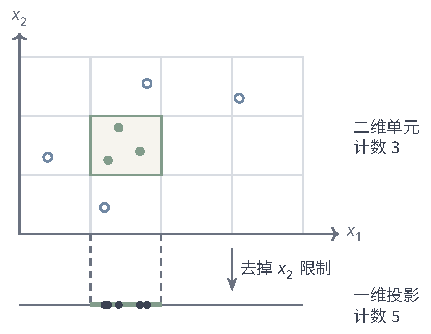
\includegraphics[width=72.912mm]{figures/04-classic-models/00-shared/tikz/clustering-subspace/figure.pdf}
  \caption{CLIQUE 的投影计数示意。二维高亮单元含三个样本，其在横轴区间上的投影还包含其他纵坐标范围的样本。取共同阈值 $\tau=3$，二维单元密集必然推出对应一维单元密集，反方向则不成立。}
 \label{fig:clustering-subspace}
\end{figure}

\subsubsection{参数学习}

CLIQUE 借鉴 Apriori 的逐层候选生成。扫描数据找到一维密集单元后，把具有兼容低维区间的单元连接成更高维候选；只有所有低一维投影都密集的候选才继续计数验证。重复直到候选为空或达到搜索维数上限。

在保留下来的子空间中，算法连接相邻密集单元，形成簇，并可用轴对齐区域的析取式压缩簇描述。原始方法还包含选择子空间和简化描述的步骤；若使用额外启发式筛选，完整性应相对于筛选后的搜索范围表述。

\subsubsection{理论分析}

\paragraph{表达能力}
CLIQUE允许客户群组只在金额和频次坐标上集中，而对年龄不加限制。它可以表达“在这两个坐标中落入某个区域”的群组，也允许同一客户在年龄子空间属于另一簇。如果目标分组还依赖被省略的年龄，那么两条所选坐标相同、年龄不同的记录在这个候选中就无法区分。子空间选择消除了无关坐标的干扰，也舍弃了这些坐标能够提供的区别。

固定子空间后，候选区域是轴对齐单元的并。网格本身对边界的逼近可以独立核验：设所选子空间有$s$个坐标，输入取值位于$[0,1]^s$，等宽网格边长为$h$，目标是其中一个闭合区域$A$。用所有与$A$相交的单元组成$A_h$，则$A\subseteq A_h$；每个多纳入的位置与$A$边界的距离至多为单元直径$\sqrt s\,h$。因此在所选坐标的分布$P_S$下，表示误差满足
\[
 P_S(A_h\mathbin{\triangle}A)
 \leq P_S\{\operatorname{dist}(\bm X_S,\partial A)
                 \leq\sqrt s\,h\}.
\]
当边界上的概率质量为零，右侧随$h\to0$趋零，说明网格可以逐步逼近该区域。CLIQUE实际只保留达到计数阈值的单元，未必恰好选到这些相交单元；细网格还会让质量分散，造成计数不足。这个几何界因而说明候选能表达多少边界细节，并未保证算法恢复$A$。

倾斜关系还会改变所需单元数。例如，二维样本沿$y=x$分布时，两个单坐标都有较大跨度，但方向$(1,-1)$上的变化可以很小。坐标子集没有这个方向；CLIQUE只能用一串较细单元覆盖斜带，再依靠连接组成簇。若要求用一个紧凑的低维方向描述群组，就需要改变候选投影，而不只是调整计数阈值。

\paragraph{收敛性}
CLIQUE 每轮增加候选的维数，最多搜索到 $d$ 维，因此在有限网格上必然结束。除了终止性，还需证明提前剪枝不会遗漏满足计数条件的高维单元；下面的向下封闭性给出这一保证。

\begin{lemma}[子空间密集性的向下封闭性]
 \label{thm:clustering-clique}
 在一致的逐维网格和共同计数阈值 $\tau$ 下，若 $S$ 上的单元 $U$ 密集，则对任意非空 $S'\subseteq S$，其投影 $U|_{S'}$ 也密集。
\end{lemma}
\begin{proof}
记 $I(U)=\{i:\bm{x}_{i,S}\in U\}$。若 $i\in I(U)$，它在 $S$ 的所有选定坐标上都满足区间限制，去掉部分坐标限制后仍然满足。因此
\[
 I(U)\subseteq I(U|_{S'}),\qquad
 n(U|_{S'})\geq n(U)\geq\tau.
\]
投影网格沿用相同区间，故 $U|_{S'}$ 是合法低维单元，并达到同一密集阈值。
\end{proof}

向下封闭性允许根据不密集的低维投影排除高维候选。多个投影各自密集时，其中的样本可能不同，所以高维计数仍需验证。该论证使用共同计数阈值；改为按体积归一的密度或随维数变化的阈值时，需重新核对剪枝条件。

有限网格保证搜索最终结束，但最坏情况下大量投影都密集，仍可能枚举指数多个子空间和单元。

\paragraph{泛化性}
CLIQUE的经验计数可以直接与总体单元质量比较。

\begin{lemma}[固定网格单元的总体质量保证]
 \label{thm:clustering-clique-mass-risk}
设样本独立同分布于$[0,1]^d$，每个坐标预先分成$\xi\geq1$个区间，所有非空坐标子集上的单元组成固定集合$\mathcal U$，其大小为
$N=(1+\xi)^d-1$。记$P_n(U)=n(U)/n$，将计数阈值写成$n t$。对任意$0<\delta<1$，Hoeffding界与并集界给出
\begin{equation}
 P_{D_n}\!\left\{
  \max_{U\in\mathcal U}|P_n(U)-P(U)|
  \leq\alpha_n
 \right\}\geq1-\delta,
 \qquad
 \alpha_n=\sqrt{\frac{\log(2N/\delta)}{2n}}.
 \label{eq:clustering-clique-mass-risk}
\end{equation}
\end{lemma}

因此每个被选中的单元都有$P(U)\geq t-\alpha_n$，每个$P(U)\geq t+\alpha_n$的单元都会被选中。这一结论同时覆盖算法检查过与尚未检查的候选，允许向下封闭剪枝在数据上选择输出。

\begin{theorem}[CLIQUE在固定网格与质量间隔下的期望判定风险界]
 \label{thm:clustering-clique-cell-risk}
若全部单元满足$|P(U)-t|\geq\gamma>0$，且
$n>\log(2N/\delta)/(2\gamma^2)$，经验与总体的密集单元集合以至少$1-\delta$的概率完全相同。固定邻接规则后，它们的连通区域也相同。将风险定义为均匀抽取一个候选单元时，经验密集判定与总体判定不一致的概率，便有
$\mathbb E_{D_n}R_{\mathrm{cell}}\leq\delta$。
\end{theorem}

这里总体目标仍是该网格及阈值定义的区域，并未保证它们对应语义类别。

阈值附近没有间隔时，式\eqref{eq:clustering-clique-mass-risk}只控制区域质量，不能排除一个临界单元改变整体连接。平移网格或自适应选择区间也改变候选集；MAFIA等方法需把这些选择计入复杂度，不能沿用预先固定网格的$N$。

\subsubsection{优化表达能力}

\paragraph{支持子空间中的非凸群组}
固定网格可能把一条密集点带切散到多个未达阈值的单元中。Kailing、Kriegel与Kr\"oger在2004年的SUBCLU中改用子空间内的DBSCAN密度连通，保留坐标子集搜索，同时让邻域连接承担区域构造\scite{clust-kailing2004}。它能在所选坐标中保留弯曲密集路径，不再要求路径逐格达到统一计数。代价是各候选子空间都需要密度查询；核心桥接与密度尺度冲突也仍然存在。

\paragraph{支持倾斜方向的群组关系}
坐标子集无法直接保留变量之间的倾斜关系。ORCLUS进一步学习任意方向的低维正交投影，把相关方向纳入候选，同时增加方向估计和矩阵计算\scite{clust-aggarwal2000}。

沿$y=x$的斜带说明二者的差别。假设$\bm X=(T,T)+\bm\eta$，$\mathbb E T=0$、$\operatorname{Var}(T)=v$，噪声$\bm\eta$独立、均值为零且协方差为$\sigma^2\bm I$。任取一个原坐标，其方差都是$v+\sigma^2$；投影到单位方向$(1,-1)/\sqrt2$，方差则只有$\sigma^2$。允许该方向的ORCLUS候选能表达由相关关系形成的低方差群组，只有坐标选择的候选无法得到同样的一维紧凑性。这个改进针对线性方向；若群组沿弯曲流形变化，一个固定线性投影仍可能把不应靠近的部分重叠，不能据此推得任意非线性结构都可恢复。

\subsubsection{优化计算能力}

\paragraph{适应各坐标的聚集尺度}
各坐标上的聚集尺度不同时，统一区间宽度可能浪费搜索，也可能把局部群体切散。Nagesh、Goil与Choudhary在2001年的MAFIA中采用自适应网格，使候选区间随数据分布调整\scite{clust-nagesh2001}。这种调整减少无效网格与候选检查，同时增加区间估计及合并的成本。区域仍由坐标区间组成，自适应宽度没有增加任意方向的投影。

\paragraph{降低紧凑子空间群组的搜索成本}
若目标是在相关坐标中寻找紧凑群体，还可以用抽样减少完整候选枚举。Procopiuc等在2002年提出DOC与FASTDOC，用随机抽样寻找包含足够多对象的投影盒子\scite{clust-procopiuc2002}。它们另行规定盒宽与群组评价，因而不是对CLIQUE搜索作等价加速。超出给定宽度的细长路径不会成为同一个紧凑候选，增大宽度又可能纳入邻近群体；抽样预算则决定哪些候选会被检查。

\subsubsection{支持子空间簇唯一归属场景}

CLIQUE允许同一对象在不同子空间获得重叠解释。若任务要求每个对象只进入一组，就需要在群组之间协调归属。\term{投影聚类}（projected clustering）通常采用硬划分，并为每簇寻找相关子空间。PROCLUS使用类似K-medoids的代表搜索，在分配与相关坐标选择之间迭代；每簇的坐标可以不同，输出却要求对象有唯一归属\scite{clust-aggarwal1999}。这会放弃一部分重叠解释，同时减少后续使用多份分组的歧义。

\subsubsection{小结}

CLIQUE适合寻找只在部分坐标上集中的群组，允许同一对象获得多个子空间解释。逐层计数筛选减少候选检查，网格与阈值则共同决定边界细节和计数是否足够。

网格边界、区间尺度与搜索规模带来不同限制。SUBCLU用密度连接减少固定网格边界的影响，MAFIA调整区间以适应局部尺度，DOC用抽样寻找另一种紧凑投影目标。若需要唯一归属或倾斜方向，则应比较投影聚类路线。它们分别增加密度查询、自适应网格、抽样或方向估计的代价，不能只根据“支持高维”选择。

\subsection{模型对比与总结}

这一组方法分别处理访问成本和相关变量选择。STING将对象汇入多层网格摘要，使区域查询不必反复访问每条记录；摘要层级较粗时，也会丢失边界细节。CLIQUE则搜索哪些坐标子集存在密集区域，回应全空间距离被无关坐标掩盖的问题，并允许同一对象获得多个子空间解释。两者都使用网格，前者侧重摘要查询，后者侧重发现相关坐标，不能仅凭数据规模决定它们可以互换。

CLIQUE的固定单元又产生边界和尺度限制。SUBCLU保留子空间搜索，用密度连接替代逐格计数，更适合相关坐标中的弯曲路径；MAFIA保留网格表示，用自适应区间回应各坐标聚集尺度不同的问题。DOC与FASTDOC另设紧凑投影盒目标，以抽样减少候选检查。它们分别改变区域构造、区间尺度和搜索对象，节省的工作与可能遗漏的结构也不同。

输出和方向是另一组区别。PROCLUS让每个对象获得唯一归属，并为不同簇选择不同坐标，适合需要一份可直接使用的划分；ORCLUS继续放宽坐标轴限制，用任意线性方向保留倾斜的低方差群组。唯一归属会放弃重叠解释，方向估计则增加参数与计算。应先确定要保留坐标关联、倾斜关系还是多份群组解释，再检查网格、距离和搜索预算。

\section{基于层次的聚类}
\label{sec:clustering-hierarchy}

探索阶段的群组粒度尚不明确时，可以保留多个层级。\term{层次聚类}（hierarchical clustering）用\term{树状图}（dendrogram）记录嵌套的合并或分裂，使分析者从同一棵树读取不同规模的划分。具体截取哪一层，仍由任务用途与证据确定。

凝聚方法从单点向上合并，分裂方法从全集向下拆分。图~\ref{fig:clustering-dendrogram}在同一棵树上读取两种粒度；截线保留已完成的层次决策，不对该粒度重新搜索。

\begin{figure}[htbp]
  \centering
  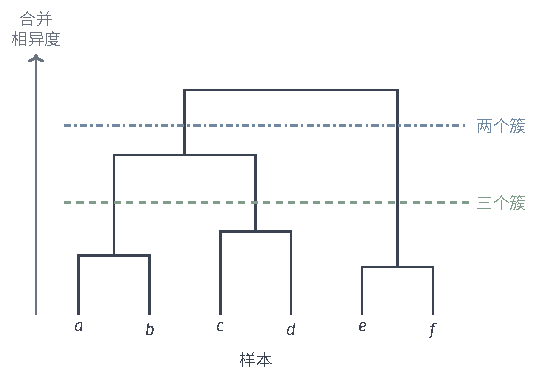
\includegraphics[width=90.914mm]{figures/04-classic-models/00-shared/tikz/clustering-dendrogram/figure.pdf}
  \caption{教学用层次树。叶节点为六个样本，内部节点高度表示合并相异度。较低截线得到三个簇，较高截线得到两个簇；图中高度为示意数值。}
 \label{fig:clustering-dendrogram}
\end{figure}

\subsection{AGNES（凝聚层次聚类）}
\label{sec:clustering-agnes}

若希望先找出最相近的客户，再观察这些小群体怎样组成较大群体，可以从每个样本各自成簇开始。\term{凝聚分析}（Agglomerative Nesting, AGNES）每次合并当前相异度最小的两簇，把合并次序与相异度保存在树中。我们可以在不同高度截取划分，无须预先固定一个$K$；已经合并的对象则不会在后续分开。Kaufman与Rousseeuw在1990年的专著中将这一长期用于数值分类学的过程与自顶向下的DIANA并列介绍。簇内出现多个样本之后，怎样定义簇间相异度就成为下一步的关键。

链接准则把不同群组偏好写进合并决策：单链接沿最近联系扩展，平均链接综合跨簇距离，Ward在1963年以最小SSE增量选择合并。凝聚方向规定构造顺序，链接准则决定哪种关系先进入树。

\subsubsection{模型结构}

初始划分为 $\mathcal{P}^{(0)}=\{\{1\},\ldots,\{n\}\}$。第 $t$ 步选择使 $D(A,B)$ 最小的两个当前簇，替换为 $A\cup B$，经过 $n-1$ 次合并得到根节点。固定相异度和确定的平局规则后，整棵树随之确定。

不同\term{链接方式}（linkage）用不同的簇间统计量：
\begin{align*}
 D_{\mathrm{single}}(A,B)
   &=\min_{i\in A,j\in B}\delta(\bm{x}_i,\bm{x}_j),\\
 D_{\mathrm{complete}}(A,B)
   &=\max_{i\in A,j\in B}\delta(\bm{x}_i,\bm{x}_j),\\
 D_{\mathrm{average}}(A,B)
   &=\frac{\sum_{i\in A,j\in B}\delta(\bm{x}_i,\bm{x}_j)}
   {|A||B|}.
\end{align*}
单链接沿近邻链扩展，可以保留细长形状，也容易被稀疏桥接点连接起来；全链接控制跨簇最远距离，倾向紧凑群组；平均链接考虑所有跨簇样本对，减弱单个极值的影响。这里的平均链接指按样本数加权的 UPGMA。

若样本处于欧氏空间，Ward 链接以合并引起的 SSE 增量定义相异度：
\[
 D_{\mathrm{Ward}}(A,B)
 =\mathrm{SSE}(A\cup B)-\mathrm{SSE}(A)-\mathrm{SSE}(B).
\]
它与 K-means 共享平方误差准则，但只允许合并已有簇。Ward 的原始工作明确以这种误差增量组织层次\scite{ward1963}。

\subsubsection{参数学习}

实现 AGNES 时，可以维护当前簇间的相异度，并在每次合并后更新相关行列。算法~\ref{alg:clustering-agnes} 省去了不影响定义的矩阵下标管理。

\begin{algorithm}[凝聚层次聚类]
 \label{alg:clustering-agnes}
 \begin{algorithmic}[1]
 \Require 样本相异度、链接方式和确定的平局规则
 \Ensure 包含合并高度的层次树
 \State 建立 $n$ 个单点簇，初始化簇间相异度
 \While{当前簇数大于 $1$}
  \State 选择使 $D(A,B)$ 最小的当前簇对
  \State 记录子簇 $A,B$ 和合并高度 $D(A,B)$
  \State 用 $A\cup B$ 替换 $A,B$
  \State 更新新簇与其他当前簇的相异度
 \EndWhile
 \end{algorithmic}
\end{algorithm}

Lance--Williams 递推使多种链接共享更新形式\scite{clust-lance1967}。
\begin{equation}
 \begin{aligned}
 D(A\cup B,C)={}&\alpha_A D(A,C)+\alpha_B D(B,C)\\
 &+\beta D(A,B)
 +\gamma|D(A,C)-D(B,C)|.
 \end{aligned}
 \label{eq:clustering-lance-williams}
\end{equation}
单链接的系数为 $(1/2,1/2,0,-1/2)$，全链接为 $(1/2,1/2,0,1/2)$，平均链接为 $(|A|/(|A|+|B|),|B|/(|A|+|B|),0,0)$。若 $D$ 直接表示 Ward 的 SSE 增量，令 $s=|A|+|B|+|C|$，则
\[
 \alpha_A=\frac{|A|+|C|}{s},\quad
 \alpha_B=\frac{|B|+|C|}{s},\quad
 \beta=-\frac{|C|}{s},\quad \gamma=0.
\]
软件也可能存储Ward增量的缩放平方根；递推系数应与其距离约定配套。

朴素实现每轮扫描全部簇对，约需$O(n^3)$时间和$O(n^2)$存储。链接结构可减少搜索：SLINK的单链接为$O(n^2)$时间和$O(n)$辅助空间，CLINK提供全链接的紧凑表示；平均、全链接和Ward的最近邻链实现也可达到$O(n^2)$时间，常见实现仍保存平方规模距离矩阵\scite{clust-muellner2011}。采用这些算法时需沿用其链接和平局约定。

\subsubsection{理论分析}

\paragraph{表达能力}
层次树能表达细群组逐步包含于粗群组的目标。它的限制也可以用四条记录说明：划分$\{\{a,b\},\{c,d\}\}$与$\{\{a,c\},\{b,d\}\}$不能同时出现在一棵树中，因为两个节点的叶集合只能互不相交或相互包含，而$\{a,b\}$与$\{a,c\}$两者都不满足。若客户按地区和按购买偏好形成交叉群组，一棵嵌套树不能同时完整保留两套关系，需要选择其中一种组织方式或改用重叠输出。

同一粒度下能否表达目标，还取决于链接准则。单链接在高度$h$截取时，得到的是距离不超过$h$的邻接图连通分量；目标若满足簇内有这样的路径、簇间没有这样的边，就会被准确保留，形状可以非凸。加入一串间距不超过$h$的桥接点，又会迫使两端合并。全链接在高度$h$形成的每簇直径不超过$h$，因为每次合并要求所有跨簇距离不超过$h$；因此不能将直径大于$h$的完整环形目标保留为一簇。平均链接综合跨簇距离，不提供同样的直径约束。Ward限定每次合并的平方失真增量，并非逐粒度重新求最小SSE。

\paragraph{收敛性}
AGNES每次合并使簇数减一，因而有限终止。要解释优化性质，还需确定链接所比较的目标；下面证明Ward对当前下一次合并的最优性。

\begin{lemma}[Ward 合并的贪心最优性]
 \label{thm:clustering-ward}
 对欧氏样本的任一当前划分，Ward 链接选择使下一步总 SSE 增量最小的簇对；任意两个非空簇满足
 \[
 \Delta\mathrm{SSE}(A,B)
 =\frac{|A||B|}{|A|+|B|}
   \lVert\bm{\mu}_A-\bm{\mu}_B\rVert_2^2.
 \]
\end{lemma}
\begin{proof}
令 $a=|A|$、$b=|B|$，则合并均值为 $\bm{\mu}=(a\bm{\mu}_A+b\bm{\mu}_B)/(a+b)$。由式~\eqref{eq:clustering-mean-decomposition}，合并后的 SSE 等于两簇原有 SSE 加上
\[
 a\lVert\bm{\mu}_A-\bm{\mu}\rVert_2^2+
 b\lVert\bm{\mu}_B-\bm{\mu}\rVert_2^2.
\]
又有 $\bm{\mu}_A-\bm{\mu}=b(\bm{\mu}_A-\bm{\mu}_B)/(a+b)$，另一项为其相反方向的 $a/b$ 倍。代入后系数为 $(ab^2+ba^2)/(a+b)^2=ab/(a+b)$。其他簇不变，因此选择最小 Ward 相异度恰好最小化当前总 SSE 增量。
\end{proof}

Ward的最优性范围是当前可合并的簇对。截取$K$簇后，若再允许样本重新分配，可继续用K-means降低SSE；此时搜索范围已从合并已有簇扩展为逐点分配，因此结果可以不同。

单链接可由完整加权图的最小生成树解释：按边权递增连接，得到同一阈值连通结构，等权边可对应不同二叉表示。全链接比较跨簇最大距离，Ward比较总平方误差增量；各准则优化当前合并，整棵树由这些局部选择累积形成。

\paragraph{泛化性}
AGNES与DIANA输出当前对象的层次树，树上没有预先定义的独立新点损失。重采样中重复出现的分支可以作为稳定性证据，仍不能替代期望风险界；相异度接近的早期合并尤其可能改变后续树形。

若用途是将新点分配给某一截取层，可以明确规定一个可检验的扩展：保留$K$个簇的均值，冻结它们，并对新点按最近均值分配。对$\lVert\bm X\rVert_2\leq r$的独立同分布欧氏样本，这一学习器的量化风险满足式\eqref{eq:clustering-kmeans-risk}，其中$e_n$是所保留中心的经验最近中心损失与全局最优量化损失之差。树的原成员未必等于最近中心分配，所以该式评价冻结中心的预测规则，不能直接评价树上每个分支。Ward的贪心合并、二分K-means及BIRCH后的中心压缩都可能影响$e_n$，并未改变经验偏差项。

\subsubsection{优化表达能力}

\paragraph{保留非球形群组的边缘结构}
用单个中心合并两个弯曲或拉长的群组，可能漏掉它们实际相邻的边缘；只用最近样本，又可能被一两个孤立点连接起来。CURE在两者之间取折中，用多个分散代表点覆盖每簇的不同部分，再把这些点向均值收缩，以减弱极端位置的影响\scite{clust-guha1998}。选择代表时，先选离均值较远的点，再逐个选择离已有代表集合较远的点。若原代表为$\bm{r}$、簇均值为$\bm{\mu}_C$，收缩后的代表可写为
\[
 \bm{r}'=(1-\alpha)\bm{r}+\alpha\bm{\mu}_C,
 \qquad 0\leq\alpha\leq1.
\]
两个簇的代表之间的最近距离用于决定合并。$\alpha=0$ 保留边缘形状，也更易受极端点影响；$\alpha$ 接近 1 时，代表逐渐退化为中心。CURE用抽样和分区减少参与完整层次搜索的对象，成本需同时计入抽样分配、代表更新及实际合并规模。

CURE增加了描述簇边缘的位置，因而可以在代表覆盖充分时比较细长或弯曲群组的局部间隔。它仍只能看见所选代表，未被代表覆盖的细小分支可能不参与合并判断。收缩也会改变目标间隔：若两圈的均值都为圆心，$\alpha=1$时所有代表都退到同一点，原本分离的两个环便无法靠代表距离区分。多个代表缓解单中心限制，代表数和收缩量则决定保留了多少形状信息。

\paragraph{适应不同群组的内部连接尺度}
群组内部的疏密不同，还会使统一的绝对距离阈值难以决定合并：对一个稠密簇很远的间隔，对稀疏簇可能只是通常的间隔。Chameleon先在近邻图上形成子簇，再把簇间连接和距离与各簇内部的对应量比较，按相对互连度与相对相近度合并\scite{clust-karypis1999}。它让合并判断随群组内部结构调整，已完成合并仍限制后续层次。

这让簇内通常间隔较大的稀疏区域不必与稠密区域使用同一个绝对合并尺度。收益成立的前提是初始子簇与近邻图保留了这些内部结构；被初始划分切断的连接或错误加入的跨群组强边，会改变随后比较的相对量。合并阶段只能组合已有子簇，若一个子簇已经混入两个目标群组，就不能再将它们分开。

\paragraph{利用类别属性的共同邻居}
对于类别属性，两条客户记录可能只共享少量属性，却与同一批其他记录相似。ROCK把这种共同支持纳入合并依据，用共同邻居形成的链接数量替代单纯点间距离，其工作发表于1999年\scite{clust-guha1999}。共享邻居能补充直接相似度，但邻居怎样定义仍决定哪些支持会被计入，也带来额外统计成本。

例如，两条记录没有直接邻接，但各自的邻居集合有三个共同对象，链接计数就保留了这份间接关系；若共同邻居为空，单凭这一对的链接则不能区分“同群体的两条孤立记录”与“不相关记录”。ROCK所能利用的目标结构必须反映在邻居重叠中。共享一个高连接对象还可能给不同群组增加共同支持，不能把共同邻居多直接解释为语义同类。

\subsubsection{优化计算能力}

层次搜索若直接保存全部对象及大量点对距离，数据装不进内存时就难以执行。Zhang、Ramakrishnan与Livny在1996年的BIRCH中先把邻近对象汇为可合并的摘要，再对摘要作聚类。它主要减少进入后续搜索的对象数，可以搭配相应的凝聚过程，而不是改变所有层次方法的目标。它用\term{聚类特征}（clustering feature, CF）记录样本数、向量和与平方范数和\scite{clust-zhang1996}。这些摘要写为
\[
 \mathrm{CF}(C)=
 \left(|C|,\ \sum_{i\in C}\bm{x}_i,\
 \sum_{i\in C}\lVert\bm{x}_i\rVert_2^2\right).
\]
这些量可相加，也可恢复均值和簇内平方误差。CF树将邻近样本汇入摘要，再对叶摘要聚类。树高和摘要规模受控时，扫描成本近似随$n$线性增长；摘要阈值、插入顺序及压缩损失共同影响最终划分。

CF对均值与SSE是充分的摘要，却不是对簇形状的完整表示。以一维教学例说明：$\{-1,-1,1,1\}$与$\{-\sqrt2,0,0,\sqrt2\}$都得到$\mathrm{CF}=(4,0,4)$，前者集中在两个位置，后者集中在三个位置。若各自被压成一个叶摘要，后续只读取CF就无法区分这两种结构，更不能根据其中的间隔重新拆出目标群组。保留更多叶摘要可以增加空间细节，同时增加内存和后续搜索。

\subsubsection{小结}

AGNES逐次合并已有群组，适合希望保留从细到粗嵌套关系的探索。链接准则决定一次合并看哪种关系：单链接关注局部连接，全链接限制最远跨度，Ward关注平方重构代价。不可撤销的合并使早期误合并传到后续层级，换一个链接并不能消除这项限制。

数据规模与簇形状可以分别处理。BIRCH先压缩对象，减少完整层次搜索的规模；CURE用多个收缩代表保留更多边缘位置；ROCK与Chameleon则改变合并所依据的关系。摘要可能损失细节，代表需要更新，关系图需要构造，这些代价应与当前距离存储和合并预算一起比较。

\subsection{DIANA（分裂层次聚类）}

有时我们更关心“整个数据先分成哪几大部分”，而非最先配对的几个样本。\term{分裂分析}（Divisive Analysis, DIANA）从所有样本组成的一簇开始，优先拆分内部差异最大的群组，再继续细分。与AGNES从局部相近关系向上合并相比，DIANA从整体差异向下建立层次；它采用的贪心拆分并不等于反向执行AGNES，早期分开的样本也不会在后续重新合并。

\subsubsection{模型结构}

DIANA 通常用簇直径 $\max_{i,j\in C}\delta(\bm{x}_i,\bm{x}_j)$ 选择待分裂簇。每次把一个非单点簇拆成两个非空子簇；若展开完整树，恰需 $n-1$ 次分裂。若只需少数大簇，也可提前停止。

\subsubsection{参数学习}

对含 $m$ 个样本的簇，非平凡无序二分共有 $2^{m-1}-1$ 种，完整枚举很快变得昂贵。DIANA 用\term{分裂群}（splinter group）贪心构造二分：选取对其余样本平均相异度最大的样本作为种子，令其自成集合 $S$，其余样本组成 $R$。

对每个 $i\in R$，在 $|R|>1$ 时计算
\[
 a_i=\frac{1}{|R|-1}\sum_{\substack{j\in R\\j\ne i}}
 \delta(\bm{x}_i,\bm{x}_j),\qquad
 b_i=\frac{1}{|S|}\sum_{j\in S}\delta(\bm{x}_i,\bm{x}_j).
\]
若最大的 $a_i-b_i$ 为正，就把对应样本从 $R$ 移到 $S$，再更新这些量；否则结束分裂。这样每一步都选择更接近分裂群的最强候选，而非按任意顺序一次扫描。保留至少一个样本在 $R$ 中，避免产生空子簇。

\subsubsection{理论分析}

\paragraph{表达能力}
DIANA的候选也服从同一嵌套限制，改变构造方向并不会让交叉分组同时进入一棵树。若目标的一个群组被第一次分裂分在两边，继续细分便不能将它重组。反过来，目标若按内部差异逐级细化，树可以保留相应层级；具体分裂群规则能否找到这些层级，还取决于相异度和贪心选择，并非由二分候选数量足够多就能保证。



\paragraph{收敛性}
每次分裂保留两个非空子簇，所以完整树恰有$n-1$次分裂。大小为$m$的待分裂簇中，分裂群已有一个种子，每次只把一个对象移入且不移回，最多再移动$m-2$个对象。两层循环因此都有限。有限二分候选中存在最优者，但分裂群启发式不枚举它们，也没有对某个全树最优目标的收敛保证。

\paragraph{泛化性}
若要评价新点，可在预定的$K$簇层截取树，保留各簇均值，并冻结最近均值预测规则。对独立同分布且范数不超过$r$的欧氏输入，其期望量化风险满足式\eqref{eq:clustering-kmeans-risk}；$e_n$是这些均值的经验最近中心损失与全局最优量化损失之差。这个结论随$n$控制抽样误差，同时保留贪心拆分造成的差距。它评价的是截取后增加的新点规则，并未把整棵层次树的分支稳定性改写为风险保证。

\subsubsection{小结}

DIANA以分裂群启发式减少二分穷举，优先提供顶层结构。相异度、种子和平局影响分裂，距离缓存、簇规模与更新方式影响成本。比较AGNES时，应在相同数据与稳定性协议下检查关键群组，而非仅凭搜索方向推断哪种更稳。

\subsection{模型对比与总结}

AGNES与DIANA都保留嵌套群组，区别在怎样构造这棵树。AGNES从单个对象逐步合并，链接准则决定先保留近邻连接、紧凑团块还是平方误差较小的合并；DIANA从全体对象逐步分裂，用分裂群启发式避免枚举所有二分，先提供顶层区别。改变方向并没有允许后续撤销已完成的分支：希望保留的群组一旦被早期操作分开或混合，后续粒度选择就会受限。

大样本和复杂形状要求在凝聚前后做不同调整。BIRCH先压缩邻近对象，使后续搜索处理较少摘要；CURE用多个收缩代表补充单中心遗漏的簇边缘。前者优先减少对象访问，后者优先保留形状，摘要阈值、代表数和收缩量也分别控制信息损失。它们可以降低大样本搜索成本，仍需检查稀少群体和细小分支有没有进入摘要或代表。

关系与尺度差异则改变合并依据。ROCK用共同邻居补充类别对象的间接相似关系；Chameleon把跨簇联系与簇内结构比较，避免稠密和稀疏区域共用一个绝对合并尺度。它们都需要可靠的初始关系，图中错误连接可能被后续合并放大。这些路线是在不同环节调整层次构造，并非一串按年份替代前人的方法。

若任务还要求估计对象来自某个生成成分的概率，层次树本身没有规定这一概率，需要进一步建立与数据相符的生成模型。

\section{基于概率的聚类}
\label{sec:clustering-probabilistic}

中心、密度连通与图割规定了群组结构。若任务还要求估计新样本来自某种群体的概率，可以假设样本先选择潜在成分，再由该成分分布生成。概率聚类据此共同估计分布参数和成分归属后验。

生成模型支持软归属、预测密度与模型比较。其成分含义需与任务群组核对：一个复杂形状的群体可能需要多个高斯近似，因此拟合密度所需的成分数与语义类别数可以不同。

\subsection{高斯混合模型（GMM）}
\label{sec:clustering-gmm}

考虑两个椭圆状的客户群组：一组沿消费金额方向伸展，另一组沿购买频次方向伸展。离两个中心同样远的记录，在前一组的主要变化方向上可能很常见，在后一组的窄方向上却很罕见。只比较中心的欧氏距离没有表达这种区别。\term{高斯混合模型}（Gaussian Mixture Model, GMM）为每个成分设置均值、协方差与权重，用它们共同计算样本的密度及成分归属概率。协方差描述各方向的伸展程度，权重描述成分在总体中的比例；重叠区域内的样本可以同时对多个成分有非零后验概率。现代教材常结合EM说明其估计\scite{bishop2006}。

Pearson 在 1894 年的研究中，用两个正态分布的混合拟合一组生物测量数据，并通过矩方程估计参数\scite{clust-pearson1894}。关键想法是：观测到的一个总体，可能混合了多个未被直接标注的子总体。分布中的多个成分因此可以作为隐含群组的统计表示。

Wolfe在1970年将多元混合分析用于模式聚类，连接多维成分表示与似然估计\scite{clust-wolfe1970}。Dempster、Laird与Rubin在1977年提出一般EM框架，处理潜变量未观测时的参数更新。GMM规定生成分布，EM规定如何估计，两者可以分别改变。

GMM同时使用均值、协方差和成分权重。协方差决定偏离均值的方向尺度，权重决定成分的相对比例；样本归属由这些量的共同密度贡献确定，软后验因此包含比中心距离更多的信息。

\subsubsection{模型结构}

与第\ref{sec:classification-gda}节的 GDA 相比，两者都用高斯密度描述输入，但 GDA 的类别标签已经观测，可以按类直接估计；GMM 的成分归属不可观测，需要作为潜在成分变量推断。具体而言，先按权重 $\pi_k\geq0$、$\sum_k\pi_k=1$ 抽取潜在成分变量 $z_i\in\{1,\ldots,K\}$，再从 $\mathcal{N}(\bm{\mu}_{z_i},\bm{\Sigma}_{z_i})$ 抽取样本。要求 $\bm{\Sigma}_k\succ0$，边际密度为
\begin{equation}
 p(\bm{x};\bm{\theta})
 =\sum_{k=1}^K\pi_k
   \mathcal{N}(\bm{x};\bm{\mu}_k,\bm{\Sigma}_k),
 \label{eq:clustering-gmm}
\end{equation}
其中 $\bm{\theta}$ 汇集权重、均值与协方差。独立同分布样本的对数似然为
\[
 \ell(\bm{\theta})
 =\sum_{i=1}^n\log\left[
 \sum_{k=1}^K\pi_k
 \mathcal{N}(\bm{x}_i;\bm{\mu}_k,\bm{\Sigma}_k)\right].
\]
求和藏在对数内，使每个成分的参数无法独立优化。

给定参数后，贝叶斯公式给出\term{责任度}（responsibility），即当前模型认为样本由某成分产生的后验概率：
\begin{equation}
 \gamma_{i,k}
 =\frac{\pi_k\mathcal{N}(\bm{x}_i;\bm{\mu}_k,\bm{\Sigma}_k)}
 {\sum_{j=1}^K\pi_j
       \mathcal{N}(\bm{x}_i;\bm{\mu}_j,\bm{\Sigma}_j)}.
 \label{eq:clustering-responsibility}
\end{equation}
责任度每行和为1，可作为软归属；硬划分取$\argmax_k\gamma_{i,k}$并处理平局。概率含义对应当前生成模型中的成分，解释为任务类别还需核对模型与语义的关系。

图~\ref{fig:clustering-gmm-responsibilities}固定两成分模型。上图相加各加权密度，得到观测总密度；下图把各成分贡献除以总密度，得到$\gamma_k(x)=p(z=k\mid x;\bm{\theta})$。对称点$x=0$的责任度各为一半，其他位置连续变化。成分归属与总密度的峰数描述不同结构，两成分混合也可能只有一个峰。

\begin{figure}[tbp]
  \centering
  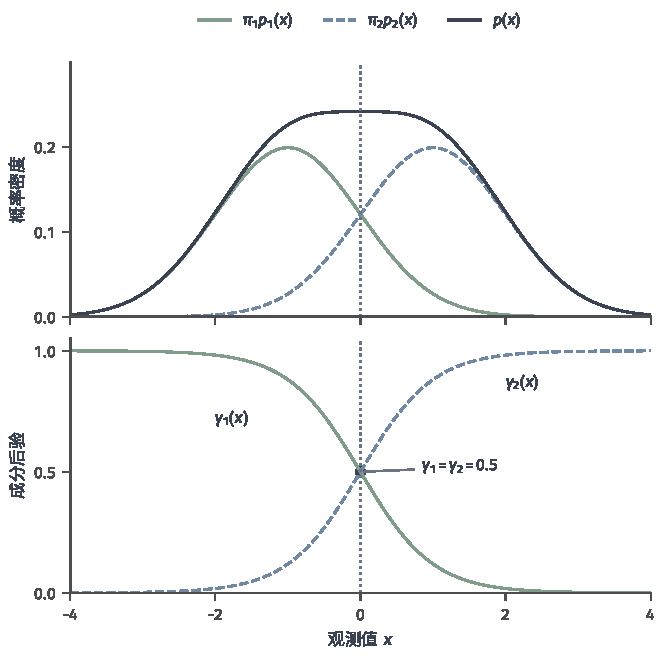
\includegraphics[width=105.412mm]{figures/04-classic-models/00-shared/matplotlib/clustering-gmm-responsibilities/figure.pdf}
  \caption{两成分 GMM 的密度与软归属。设 $\pi_1=\pi_2=1/2$、$\mu_1=-1$、$\mu_2=1$，两个方差均为 1，$p_k(x)$ 表示第 $k$ 个高斯密度。上图展示加权成分密度及其和，下图展示同一观测值对应的后验；颜色与线型在两图中保持一致。}
 \label{fig:clustering-gmm-responsibilities}
\end{figure}

\subsubsection{参数学习}

\term{期望最大化}（Expectation-Maximization, EM）交替估计潜在成分变量的分布和优化参数，Dempster、Laird 与 Rubin 将这一原则统一为一般框架\scite{clust-dempster1977}。E 步用当前参数 $\bm{\theta}^{(t)}$ 计算式~\eqref{eq:clustering-responsibility}；M 步固定这些责任度，最大化完全数据对数似然的期望。潜在成分变量不再藏在对数的求和中，而是通过 E 步给出的分布参与加权。

忽略与参数无关的常数，M 步目标为
\begin{equation}
 \begin{aligned}
 Q(\bm{\theta}\mid\bm{\theta}^{(t)})
 =\sum_{i,k}\gamma_{i,k}^{(t)}
 \biggl[&\log\pi_k-\frac12\log\det\bm{\Sigma}_k\\
 &-\frac12(\bm{x}_i-\bm{\mu}_k)^\top
 \bm{\Sigma}_k^{-1}(\bm{x}_i-\bm{\mu}_k)\biggr].
 \end{aligned}
 \label{eq:clustering-gmm-q}
\end{equation}
M步把责任度看作固定的样本权重，分别重新估计成分比例、均值和协方差。记有效样本量$n_k^{(t)}=\sum_i\gamma_{i,k}^{(t)}$。对于成分比例，在$\sum_k\pi_k=1$的约束下最大化$\sum_k n_k^{(t)}\log\pi_k$；加入拉格朗日乘子后，驻点满足$n_k^{(t)}/\pi_k=\lambda$，再对$k$求和得到$\lambda=n$。对于均值，$Q$中的相关项是责任度加权的负平方Mahalanobis距离。令其对$\bm\mu_k$的梯度为零，消去公共的正定因子$\bm\Sigma_k^{-1}$，就得到加权残差和为零。因此，这两项更新分别为
\begin{equation}
 \pi_k^{(t+1)}=\frac{n_k^{(t)}}{n},\qquad
 \bm{\mu}_k^{(t+1)}
 =\frac{\sum_i\gamma_{i,k}^{(t)}\bm{x}_i}{n_k^{(t)}}.
 \label{eq:clustering-gmm-mean}
\end{equation}
每个样本按其责任度贡献一部分计数与观测值，硬分配中的簇规模和簇均值由此变为有效样本量与加权均值。

再令精度矩阵 $\bm{\Lambda}_k=\bm{\Sigma}_k^{-1}$，加权散布为
\[
 \bm{S}_k=\sum_i\gamma_{i,k}^{(t)}
 (\bm{x}_i-\bm{\mu}_k^{(t+1)})
 (\bm{x}_i-\bm{\mu}_k^{(t+1)})^\top.
\]
把协方差改写为精度矩阵后，$Q$中需要最大化的部分为$\tfrac12[n_k^{(t)}\log\det\bm{\Lambda}_k-\operatorname{tr}(\bm{\Lambda}_k\bm{S}_k)]$。令这一部分的矩阵梯度为零，得到$n_k^{(t)}\bm{\Lambda}_k^{-1}-\bm{S}_k=\bm{0}$；换回协方差，就得到加权散布除以有效样本量：
\begin{equation}
 \bm{\Sigma}_k^{(t+1)}
 =\frac{\bm{S}_k}{n_k^{(t)}}.
 \label{eq:clustering-gmm-covariance}
\end{equation}
更新要求有效样本量为正。加权散布正定时，无约束协方差取得正定域内的有限最优；退化散布则需要协方差约束或其他估计。

代码~\ref{code:clustering-gmm}在对数域计算责任度，并用协方差特征值下界$\epsilon$避免塌缩。该截断求解固定约束$\bm{\Sigma}_k\succeq\epsilon\bm{I}$下的M步；每轮任意加常数矩阵则对应另一种估计，需另说明目标。

\begin{codeblock}[language=Python,label={code:clustering-gmm}]{带协方差下界的 GMM--EM}
import numpy as np
from scipy.special import logsumexp
from scipy.stats import multivariate_normal

def gmm_em(X, K, max_iter=100, tol=1e-5, eps=1e-6):
    X = np.asarray(X, dtype=float)
    n, d = X.shape
    if eps <= 0:
        raise ValueError("eps must be positive")
    _, mu = kmeans(X, K)
    pi = np.full(K, 1.0 / K)
    cov = np.repeat((max(1., eps) * np.eye(d))[None], K, axis=0)
    def e_step():
        log_p = np.column_stack([
            np.log(pi[k]) + multivariate_normal.logpdf(
                X, mean=mu[k], cov=cov[k])
            for k in range(K)])
        normalizer = logsumexp(log_p, axis=1)
        gamma = np.exp(log_p - normalizer[:, None])
        return gamma, normalizer.sum()
    gamma, ll = e_step()
    for _ in range(max_iter):
        nk = gamma.sum(0)
        if (nk <= 0).any():
            raise ValueError("numerically empty component")
        pi = nk / n
        mu = (gamma.T @ X) / nk[:, None]
        for k in range(K):
            diff = X - mu[k]
            S = (diff * gamma[:, k, None]).T @ diff / nk[k]
            values, vectors = np.linalg.eigh(S)
            cov[k] = (vectors * np.maximum(values, eps)) @ vectors.T
        gamma, new_ll = e_step()
        if abs(new_ll - ll) <= tol * (1 + abs(ll)):
            break
        ll = new_ll
    return pi, mu, cov, gamma
\end{codeblock}

该实现调用前文的 K-means，以其中心初始化，返回的责任度由最终参数重新计算。协方差特征值截断之所以是上述受限 M 步的解，是因为最优协方差与加权散布共享特征向量，每个特征值分别最小化 $\log s+\lambda/s$，在 $s\geq\epsilon$ 上得到 $s=\max\{\lambda,\epsilon\}$。计算中可同时记录似然变化、不同重启的目标和近空成分，以检查数值误差及初始化影响。

完整协方差保留全部二阶方向关系；类内有效样本不足时，可采用对角、球形或共享协方差减少自由度。完整形式一轮约需$O(nKd^2+Kd^3)$运算，立方项来自矩阵分解，对角形式的主要成本为$O(nKd)$。K-means++、重启和初始划分协方差可提供不同起点，其结果在同一约束与似然下比较。

\subsubsection{理论分析}

\paragraph{表达能力}
GMM要逼近的是输入密度，成分后验再由这个密度表示决定。若总体确由$K$个满足候选协方差条件的高斯成分混合生成，真密度就在候选族中，可以达到零KL逼近误差。反过来，一个高斯只能形成一个椭圆状密度峰；每个非退化高斯在全空间为正，有限混合也不能精确表示具有正测度零密度区域的目标，尾部仍不能等同于幂律等重尾分布。增加成分可以改善这些分布的近似，却不等于消除了固定$K$的失配。

协方差限制带来的误差也可以明确计算。假设二维目标是均值为零、协方差为
\[
 \bm\Sigma_\star=
 \begin{pmatrix}1&\rho\\\rho&1\end{pmatrix},
 \qquad 0<|\rho|<1
\]
的高斯分布。一个完整协方差成分可以准确表达它；若只允许一个对角协方差成分，最优均值仍为零、两个最优方差仍为1，但最小KL误差为
\[
 \inf_{\bm\mu,\,\bm\Sigma\text{ 对角}}
 D_{\mathrm{KL}}\bigl(\mathcal N(\bm0,\bm\Sigma_\star)
                 \Vert\mathcal N(\bm\mu,\bm\Sigma)\bigr)
 =-\tfrac12\log(1-\rho^2)>0.
\]
这是将高斯对数密度对目标取期望后，分别最小化均值项和两个方差项得到的结果；遗漏的相关方向由行列式$1-\rho^2$留下误差。多个对角成分可以用不同位置补充这种相关形状，但此时增加的是成分数，不能把单成分限制的结论直接套给整个混合族。

允许成分数增加时，密度逼近可以由一个具体构造说明。设$f$是$\mathbb R^d$上连续且具有紧支撑的概率密度，$\varphi_\sigma$为协方差$\sigma^2\bm I$的零均值高斯密度。把支撑划成直径不超过$\Delta$的有限单元，在每个单元$U_j$内选一个位置$\bm\mu_j$，并令$\pi_j=\int_{U_j}f$。将零质量单元略去，得到合法混合
\[
 p_{\sigma,\Delta}(\bm x)
 =\sum_j\pi_j\varphi_\sigma(\bm x-\bm\mu_j).
\]
先以卷积平滑$f$，再把每个单元中的连续中心移到$\bm\mu_j$，两步误差满足
\[
 \lVert f-p_{\sigma,\Delta}\rVert_{L^1}
 \leq\lVert f-f*\varphi_\sigma\rVert_{L^1}
       +\sqrt{2/\pi}\,\Delta/\sigma.
\]
第二项来自高斯密度沿位移方向的导数积分：两个同协方差高斯的$L^1$距离不超过$\sqrt{2/\pi}$乘以均值距离再除以$\sigma$。第一项随$\sigma\to0$趋零，因为密度平移的$L^1$差趋零，卷积只是在高斯位移下平均这些差。故选择$\sigma\to0$、$\Delta/\sigma\to0$，有限混合就能把这类目标的$L^1$误差降到任意小。这个结论允许成分数增加、方差缩小，不适用于固定$K$或固定正方差下界的候选族，也未给出KL误差或语义簇恢复保证。一个弯曲群体可能需要沿其形状布置多个高斯，因而密度拟合所需的成分数可以大于群体数。

\paragraph{收敛性}
EM在旧参数处构造与观测似然相等的下界，再提高这一辅助目标。这样可避免直接优化对数内的成分求和；精确E步与M步改进条件共同给出似然不下降。

\begin{theorem}[GMM的精确EM迭代的似然上升性质]
 \label{thm:clustering-em}
 E 步取当前精确后验，M 步满足
 $Q(\bm{\theta}^{(t+1)}\mid\bm{\theta}^{(t)})
 \geq Q(\bm{\theta}^{(t)}\mid\bm{\theta}^{(t)})$。
 在相关概率与期望有限、支持条件允许下，则
 $\ell(\bm{\theta}^{(t+1)})\geq\ell(\bm{\theta}^{(t)})$。
\end{theorem}
\begin{proof}
对每个样本，令$q_i$相对于当前参数下成分后验的KL散度有限，直接使用整体对数比形式（参考\BookSectionRef{sec:information-elbo-approximation}{卷2《数学准备：概率、因果与决策》第2章“概率分布”第2.5.2节“表示约束下的分布逼近”}）：
\[
 \begin{aligned}
 \mathcal L_i(q_i,\bm\theta)
 &=\sum_{k:q_i(k)>0}q_i(k)
    \log\frac{p(\bm x_i,z_i=k;\bm\theta)}{q_i(k)},\\
 \log p(\bm x_i;\bm\theta)
 &=\mathcal L_i(q_i,\bm\theta)
   +D_{\mathrm{KL}}\bigl(q_i\Vert p(z_i\mid\bm x_i;\bm\theta)\bigr).
 \end{aligned}
\]
对样本求和，把下界记为$\mathcal L(q,\bm\theta)$。该分解不要求$q_i$覆盖后验的全部支撑；
若改用恢复证据的Jensen等式，则必须另查相反方向的覆盖条件。
E 步令 $q_i^{(t)}$ 等于旧参数的后验，因此 $\mathcal{L}(q^{(t)},\bm{\theta}^{(t)})=\ell(\bm{\theta}^{(t)})$。固定 $q^{(t)}$ 后，下界与 $Q$ 仅相差不含参数的熵项，M 步遂给出
\[
 \begin{aligned}
 \ell(\bm{\theta}^{(t+1)})
 &\geq\mathcal{L}(q^{(t)},\bm{\theta}^{(t+1)})\\
 &\geq\mathcal{L}(q^{(t)},\bm{\theta}^{(t)})
 =\ell(\bm{\theta}^{(t)}).
 \end{aligned}
\]
这就证明了单调性。
\end{proof}

似然有上界时，EM的单调性可进一步给出似然值收敛。参数趋于驻点还需连续性、紧性等正则条件，Wu给出了相应分析\scite{clust-wu1983}。驻点可能是局部极大值或鞍点，优化解释应分别核对值的极限、参数极限和驻点类型。

当 $K\geq2$，且模型中存在一个可塌缩的正权重成分，其余正权重成分仍使其他样本的混合密度保持正值时，无约束 GMM 的似然没有上界。令可塌缩成分的均值等于某个样本，协方差为 $\sigma^2\bm{I}$；当 $\sigma\to0$ 时，该样本处的密度按 $\sigma^{-d}$ 增长，而其他样本仍由其余成分覆盖，因此总对数似然可以无界增加。若 $K=1$ 且样本经验散布矩阵正定，单高斯的最大似然有限；若经验散布矩阵奇异，协方差仍可能在数据未占据的方向趋近边界并导致似然退化。协方差下界、适当先验或惩罚可以阻止这类塌缩，但它们各自改变了优化问题。

潜在成分编号的置换不改变混合密度；当成分彼此不同且权重为正时，一个解通常对应 $K!$ 个等价标号。这与不同拟合质量的局部极值是两类问题。

\paragraph{泛化性}
GMM可以为新观测给出密度，因此以对数损失评价泛化：
$R(\bm\theta)=\mathbb E_P[-\log p_{\bm\theta}(\bm X)]$，
$\widehat R_n=-\ell(\bm\theta)/n$。
无约束似然可以塌缩，下面明确采用有界的候选族，而不把EM的似然上升当作统计保证。

\begin{theorem}[GMM在有界参数与非退化协方差下的期望对数风险界]
 \label{thm:clustering-gmm-risk}
设训练样本独立同分布于$P$，$\lVert\bm X\rVert_2\leq r$几乎处处，固定$K$，并在训练前规定
$\lVert\bm\mu_k\rVert_2\leq A$、$a\bm I\preceq\bm\Sigma_k\preceq b\bm I$，其中$0<a\leq b$；权重属于概率单纯形。用均值、权重及对称协方差的独立坐标组成参数向量，协方差坐标按Frobenius范数计量。令
\[
 \begin{aligned}
 p_0&=K+Kd+Kd(d+1)/2,\\
 B_0&=\sqrt{1+KA^2+Kdb^2},\\
 q_-&=(2\pi b)^{-d/2}e^{-(r+A)^2/(2a)},\\
 q_+&=(2\pi a)^{-d/2},\\
 M_0&=\tfrac d2\log(b/a)+\tfrac{(r+A)^2}{2a},\\
 L_0^2&=K(q_+/q_-)^2+\frac{(r+A)^2}{a^2}\\
 &\quad+\frac14\left(\frac{(r+A)^2}{a^2}+\frac{\sqrt d}{a}\right)^2.
 \end{aligned}
\]
混合密度始终介于$q_-$与$q_+$，所以对数损失的取值区间长度至多为$M_0$。均值及协方差的对数密度导数由责任度加权，权重导数则由$q_+/q_-$控制，合并得到参数Lipschitz常数$L_0$。参数集在$p_0$维半径$B_0$的球内，故其$\epsilon$覆盖数至多为$(1+2B_0/\epsilon)^{p_0}$。

对该受约束族的任意学习器，记$e_n$为经验对数损失距全局最优的差。引理\ref{thm:clustering-cover-risk}取$\epsilon=B_0/n$给出
\begin{equation}
 \begin{aligned}
 \mathbb E_{D_n}R(\widehat{\bm\theta})
 &\leq\inf_{\bm\theta\in\Theta}R(\bm\theta)
       +\frac{4L_0B_0}{n}\\
 &\quad+2M_0\sqrt{\frac{p_0\log(1+2n)+\log2}{2n}}
       +\mathbb E_{D_n}e_n.
 \end{aligned}
 \label{eq:clustering-gmm-risk}
\end{equation}
\end{theorem}

高概率版本同样将$\log2$换成$\log(2/\delta)$。约束阻止密度尖峰无限提高训练似然，并使全体候选的训练与新样本损失能够同时比较；EM的局部求解误差保留在$e_n$中。若$P$有密度且熵有限，$R(\bm\theta)-H(P)=\operatorname{KL}(P\Vert p_{\bm\theta})$，上式也给出距该族最佳密度的KL超额风险界。它允许分布失配，不要求参数或成分标号唯一，也不评价语义簇标签。

成分数与协方差形式改变候选族，需另行选择。完整协方差的自由参数数目为
\[
 m_K=(K-1)+Kd+\frac{Kd(d+1)}2,
\]
常用准则为
\begin{equation}
 \mathrm{BIC}(K)=-2\ell(\hat{\bm\theta}_K)+m_K\log n,
 \qquad
 \mathrm{AIC}(K)=-2\ell(\hat{\bm\theta}_K)+2m_K.
 \label{eq:clustering-bic}
\end{equation}
它们用较小值选择候选，并非式\eqref{eq:clustering-gmm-risk}的替代界。BIC的证据近似依赖渐近条件；有限混合存在零权重边界与奇异参数，混合阶数的一致性需核对专门条件\scite{clust-keribin2000}。将所选成分数解释为语义类别数，还需外部知识。

\subsubsection{与中心量化的联系}

GMM的软归属、权重与协方差共同定义后验，K-means只使用中心平方距离。固定部分参数并取小方差极限，可以明确两种目标和更新的联系。固定均匀权重 $\pi_k=1/K$ 和共享球形协方差 $\bm{\Sigma}_k=\sigma^2\bm{I}$，则
\[
 \gamma_{i,k}=
 \frac{\exp(-\lVert\bm{x}_i-\bm{\mu}_k\rVert_2^2/(2\sigma^2))}
 {\sum_j\exp(-\lVert\bm{x}_i-\bm{\mu}_j\rVert_2^2/(2\sigma^2))}.
\]
若 $\bm{x}_i$ 的最近中心唯一为 $k^\ast$，则对任意 $j\ne k^\ast$，距离平方差为正，相应指数比随 $\sigma^2\to0$ 趋零，故 $\gamma_{i,k^\ast}\to1$。M 步的均值更新因此退化为 Lloyd 更新；平局时责任度可分散在多个最近中心，不能直接得到唯一硬簇分配。

去掉只依赖$\sigma$的常数，目标$-2\sigma^2\ell$趋向$\sum_i\min_k\lVert\bm{x}_i-\bm{\mu}_k\rVert_2^2$，给出平方误差的联系。这一极限固定均匀权重并缩小共享球方差；自由协方差GMM优化更大的分布族。FCM的软隶属度则来自模糊损失，与生成后验采用不同定义。

\subsubsection{优化表达能力}

\paragraph{表示二值与计数分布}
高斯成分规定了连续的椭圆分布。二值与计数数据需要先改变观测机制，例如采用伯努利或多项式成分，再按相应似然计算责任度和更新参数。混合结构可以保留，单个成分所描述的关系则随分布而变。

一个按坐标独立的伯努利成分无法表达成分内部任意的二值相关性；允许参数取0或1并使用至多$2^d$个成分时，却可以分别在每个二值向量上放置所需概率质量，准确表示任意二值联合分布。多项式成分规定总计数给定后的重复类别抽取，额外的过度离散或依赖未必在单成分中。选择成分时应检查这些关系是否足以描述观测。

\paragraph{放宽预定成分数的限制}
有限混合要求先固定$K$，当成分数本身也不明确时，就需要比较不同$K$或把这一不确定性纳入模型。\term{狄利克雷过程混合}（Dirichlet process mixture, DPM）为成分参数的混合测度设置Dirichlet过程先验，让一批有限样本所使用的成分数随数据和后验变化。总质量参数控制新增成分的倾向，折棒表示及后验预测见\BookSectionRef{sec:pgm-static-directed-hierarchy-membership}{卷六“模型：概率图模型”的“层次结构与混合成员”节}；Neal研究了相应MCMC推断\scite{clust-neal2000}。它省去了固定$K$这一步，但先验仍影响成分数，成分也仍需与任务类别核对。

DPM放宽了预定有限成分数的限制，成分分布族与先验支持仍限定可表达的密度。若基分布不允许某些均值位置或足够小的方差，上述逐单元放置高斯的构造就未必位于该先验支持内。只有候选支持包含目标所需的参数和混合结构，增加潜在成分才可能降低相应逼近误差；它本身不保证后验找到该密度，更不保证使用的成分数等于语义类别数。

\subsubsection{优化泛化能力}

连续数据中若少量记录远离主体，高斯成分可能把尺度撑大，或多用一个成分专门解释这些记录。Peel与McLachlan在2000年研究的$t$混合改用较厚的尾部，在拟合中降低远离成分中心的观测对位置与尺度更新的牵动\scite{clust-peel2000}。这种调整保留混合与责任度机制，同时增加尺度及自由度处理；若远点实际属于一个重要小群体，减弱其影响也未必符合任务。$t$成分仍围绕椭圆尺度组织位置，较厚尾部没有让单个成分能够表达任意弯曲群组。

\subsubsection{小结}

GMM在同一模型中给出预测密度与成分归属后验，适合需要概率评分或生成解释的任务。协方差决定成分的方向与尺度，权重决定成分的相对质量；拟合时还要处理似然退化与局部求解。密度拟合所用的成分不必恰好对应业务类别，增加成分也会增加解释负担。

分布不合适与成分数不明确是不同问题。二值、计数或重尾成分改变每组怎样生成观测，因而要重新选择似然与参数更新；DPM则把成分数的不确定性纳入先验和后验推断，保留了成分分布及先验选择的责任。使用哪条路线，应先看误差来自观测机制、尾部还是预定的$K$，再比较新增参数与推断预算。

\subsection{模型对比与总结}

K-means以距离定义压缩误差，GMM则把观测解释为不同生成成分的混合，额外估计成分比例和协方差，并给出软归属与预测密度。共享球形协方差、均匀权重的小方差构造连接了两者；自由协方差GMM能够表达不同尺度与方向，也增加参数、似然退化和局部推断问题。需要这些几何变化或概率输出时，可以评价新增设定是否值得，不能把GMM简单视为更精细的中心划分。

成分模型沿两条方向调整。二值或计数混合改变观测取值机制，$t$混合改变连续成分的尾部，分别回应高斯成分无法描述的观测和异常值影响；责任度机制仍然保留，似然与更新需要随之改变。DPM处理的则是预先固定成分数的限制，通过先验与后验决定有限样本使用多少成分，代价在先验选择和更复杂的推断。改变成分分布与放宽成分数可以配合，不能相互替代。

概率成分也未必等于业务群组。一个弯曲群体可能需要多个高斯成分拟合，两个业务类别也可能共享同一生成规律。若目标是预测密度，就比较新样本对数损失；若目标是解释客户群体，还需检查成分与外部语义及下游用途的关系。这个区别决定了应评价拟合还是分组。

\section{半监督聚类}
\label{sec:clustering-semisupervised}

未标注数据也可能附有部分领域知识。例如，专家知道两条记录来自同一对象，知道一对样本应分开，或能给出少量典型种子。\term{半监督聚类}（semi-supervised clustering）将这些信号用于以未标注样本为主体的分组。

第\ref{sec:classification-semisupervised}节的半监督分类利用未标注输入改进预先定义类别的预测，本节则用少量类别标签或关系先验共同决定分组。两者都改变可用监督信息，却保留不同的任务目标。

实例级信号常写为\term{必连约束}（must-link）和\term{勿连约束}（cannot-link）：前者要求两个样本同簇，后者要求异簇。记其索引对集合为 $M$ 和 $B$，以免与簇 $C_k$ 或划分 $\mathcal{P}$ 混淆。信号既可作为硬约束，也可带权违反；少量关系判断是否比逐点类别标签更容易获取，取决于实际标注任务。

这些信号与几何结构共同确定群组。需要检验的是先验是否消除了原模型的歧义，覆盖了哪些样本，以及是否与基础几何发生冲突；信号质量和作用范围决定其可能收益。

\subsection{COP-K-means}
\label{sec:clustering-cop}

例如，两条记录来自同一对象的不同时间，专家要求它们同组；另两条记录已知属于不同群体，要求它们分开。普通K-means只比较到中心的距离，无法保证这些关系。COP-K-means把关系作为硬条件，每次只从不违反已有关系的簇中选择最近中心。Wagstaff等在2001年提出了这一方法\scite{clust-wagstaff2001}。平方误差目标保留，但一些距离更近的分配会被排除，约束是否可行与样本访问次序也需要处理。

\subsubsection{模型结构}

目标仍为式~\eqref{eq:clustering-sse}，可行域增加
\begin{equation}
 c_i=c_j\quad((i,j)\in M),\qquad
 c_i\ne c_j\quad((i,j)\in B).
 \label{eq:clustering-cop}
\end{equation}
must-link 的传递闭包把样本分成\term{约束块}（chunklet），同一块必须整体分配。若 cannot-link 的两端落在同一块内，约束立即矛盾；但不存在这种矛盾还不足以保证给定 $K$ 下可行。

把每个约束块当作顶点、cannot-link 当作边，块的簇分配实际上是该图的 $K$ 着色。例如三个两两 cannot-link 的块不能放进两个簇，即使没有任何 must-link 冲突。块级 SSE 可分解为块内常数加上“块大小乘以块均值到中心的平方距离”，因此整体分配也能利用摘要。

\subsubsection{参数学习}

COP-K-means 按某个顺序处理样本或约束块，对候选簇按距离排序，接受第一个与已固定分配相容的簇。若没有候选，就报告本次贪心分配失败；更新步则对每个非空簇取均值。

\begin{algorithm}[COP-K-means 的约束块分配]
 \label{alg:clustering-cop}
 \begin{algorithmic}[1]
 \Require must-link 闭包、块间 cannot-link、当前中心
 \Ensure 本轮可行分配，或本轮贪心失败
 \State 清空本轮簇分配，选定约束块访问顺序
 \For{每个约束块 $U$}
  \State 按 $\sum_{i\in U}\lVert\bm{x}_i-\bm{\mu}_k\rVert_2^2$ 排序候选簇
  \State 选择不与已分配邻块冲突的最近候选
  \If{候选不存在}
   \State 返回本轮失败
  \EndIf
  \State 把 $U$ 的全部样本分给所选簇
 \EndFor
 \end{algorithmic}
\end{algorithm}

贪心失败可能来自顺序，而非约束本身。以cannot-link路径$a-b-c-d$和$K=2$为例：按$a,d,b,c$访问，若$a,d$先取簇1，$b$只能取簇2，$c$便无可行选择。整体划分$\{a,c\}$与$\{b,d\}$却满足全部关系，说明局部已定选择阻碍了后续分配。

逐块贪心未精确求解固定中心的整体约束分配，Lloyd的下降前提在这里需要重新建立。可从已有可行解出发，只接受可行且降低目标的块移动；也可精确求解受约束分配，再更新均值。前者搜索范围较小，后者增加组合优化成本。普通COP实现可用迭代上限、失败记录及重启或回溯处理这些情况。

\subsubsection{理论分析}

\paragraph{表达能力}
这些约束缩小的是当前对象的候选划分。目标若满足全部关系，它仍然可行；只要一条错误的硬关系与目标冲突，目标就被排除。它也可以允许一些违反最近中心规则的训练分配，因此有望保留距离本身无法确定的关系，但未被约束覆盖的对象仍主要由平方距离决定。约束满足只说明这批对象的关系表达正确，不会自动给独立新点增加一个非线性分组规则。



\paragraph{收敛性}
若约束存在可行分配，有限种分配各自通过簇均值得到最小平方误差，因此整体最小值存在。普通逐块贪心分配却可能失败，也不自动满足Lloyd的下降条件。采用精确可行分配步与均值更新，并在平局时保留原分配、只接受严格改进时，有限分配数才给出有限停止保证；它仍可能停在受约束的局部解。回溯、重启或迭代上限只是求解策略，不能替代可行性证明。

\paragraph{泛化性}
为评价独立新点，冻结输出的$K$个中心，并以最近中心平方距离作为损失。若训练输入独立同分布且$\lVert\bm X\rVert_2\leq r$，中心也位于该球内，则定理\ref{thm:clustering-kmeans-risk}直接给出
\[
 \mathbb E R(\widehat{\bm\mu})\leq\inf_{\lVert\bm\mu_k\rVert_2\leq r}R(\bm\mu)
 +\frac{16r^2}{n}
 +8r^2\sqrt{\frac{Kd\log(1+2n)+\log2}{2n}}
 +\mathbb E e_n.
\]
这里$e_n$按所有球内中心的经验最近中心损失计算，保留了约束、初始化及搜索带来的差距；约束本身可以依赖训练样本，因为偏差控制同时覆盖全部中心。该结论只评价量化失真，不保证新点满足未提供的成对关系或语义标签。

\subsubsection{优化泛化能力}

若先验允许出错，PCK-means 在 SSE 上增加
\[
 \sum_{(i,j)\in M}w_{i,j}^{M}\mathbb{1}\{c_i\ne c_j\}
 +\sum_{(i,j)\in B}w_{i,j}^{B}\mathbb{1}\{c_i=c_j\},
\]
以软惩罚权衡几何和约束。有限权重不保证零违反，但避免因单条错误关系直接拒绝整个问题。

\subsubsection{小结}

COP-K-means把可靠关系作为分配条件，成功输出可以逐项核查。它要求区分先验本身冲突、给定$K$下不可行与贪心顺序失败；这些情况需要不同的诊断，不能都解释成数据没有可分群组。

关系可能出错时，PCK-means用有限惩罚允许违反，让距离拟合与监督信号共同参与取舍。这样避免了单条错误关系直接拒绝整个分配，但权重需要反映可信程度，输出也必须报告违反哪些关系。软化条件改变了目标，不能继续按硬条件解释每一对关系。

\subsection{Seeded / Constrained K-means}
\label{sec:clustering-seeded}

成对关系告诉我们哪些对象应该合在一起，却不一定告诉我们群组的名称。若每类已有少量带标签的典型记录，就可以用这些种子确定初始中心，或在整个学习过程中固定它们的类别。Basu、Banerjee与Mooney在2002年研究了Seeded K-means与类别标签约束的Constrained K-means\scite{clust-basu2002}。前者只用种子引导起点，后者让种子的类别持续参与分配条件；后者与第~\ref{sec:clustering-capacity}节限制簇容量的同名方法含义不同。

\subsubsection{模型结构}

设种子索引集合为 $S$，类别标签为 $\ell_s\in\{1,\ldots,K\}$，并记 $S_k=\{s\in S:\ell_s=k\}$。当每类都有种子时，初始化为
\[
 \bm{\mu}_k^{(0)}
 =\frac{1}{|S_k|}\sum_{s\in S_k}\bm{x}_s.
\]
缺少种子的簇需另外初始化。Seeded 版本只在初始化时使用类别标签，之后种子可以移动；Constrained 版本始终要求 $c_s=\ell_s$，把种子类别标签作为硬事实。二者都优化同一个平方误差目标，只是初始化与可行域不同。

\subsubsection{参数学习}

Seeded 版本随后直接运行 Lloyd。Constrained 版本在分配步冻结种子，其余样本独立选择最近中心；更新中心时同时计入种子和非种子。由于冻结限制彼此不耦合，逐点分配仍是固定中心下的精确最优解，因此可沿用定理~\ref{thm:clustering-lloyd} 的下降论证与平局条件。每簇都有固定种子时，还自然避免了空簇。

种子确定了部分群组的名称与初始位置，其代表性仍影响结果。允许种子移动，可以缓解错误标签的永久锁定；可靠标签与模糊几何并存时，冻结种子更能保留监督关系。选择哪种方式，应按种子覆盖、比例和错误类型，在未参与拟合的证据上比较。

\subsubsection{理论分析}

\paragraph{表达能力}
Seeded版本没有改变候选中心族，因而不会消除K-means对完整内外圆的表达限制；它改变的是算法从哪里搜索。冻结标签的版本确保被标注对象采用所需名称，却不能把相同形状保证扩展到未标注对象。若某个种子标签错误，真实目标被硬条件排除；若标签正确而目标在当前表示中不是最近中心区域，仅增加少量种子也不能使全部未标注分配吻合目标。



\paragraph{收敛性}
Seeded版本在初始化后就是Lloyd迭代。固定种子标签的版本仍能逐点精确最小化分配子问题，再由均值精确最小化中心子问题，因此同样满足定理\ref{thm:clustering-lloyd}的下降结论。在非空簇、固定平局规则且只接受严格改进的条件下，有限分配给出有限停止；每类具有固定种子可以保证非空。最优分配存在，但从种子起点运行并不保证找到全局最优解。

\paragraph{泛化性}
为评价独立新点，冻结输出的$K$个中心，并以最近中心平方距离作为损失。若训练输入独立同分布且$\lVert\bm X\rVert_2\leq r$，中心也位于该球内，则定理\ref{thm:clustering-kmeans-risk}直接给出
\[
 \mathbb E R(\widehat{\bm\mu})\leq\inf_{\lVert\bm\mu_k\rVert_2\leq r}R(\bm\mu)
 +\frac{16r^2}{n}
 +8r^2\sqrt{\frac{Kd\log(1+2n)+\log2}{2n}}
 +\mathbb E e_n.
\]
这里$e_n$按所有球内中心的经验最近中心损失计算，保留了约束、初始化及搜索带来的差距；约束本身可以依赖训练样本，因为偏差控制同时覆盖全部中心。该结论只评价量化失真，不保证新点满足未提供的成对关系或语义标签。

\subsubsection{小结}

种子方法通过初始化或固定归属引入少量类别标签，适合每类已有代表样本的任务。距离与均值继续规定几何；若监督还需改变特征方向的重要性，可以进一步学习度量。

\subsection{MPCK-means}
\label{sec:clustering-mpck}

继续以客户金额、频次和年龄为例。专家认为两名年龄相差很大的客户应归为一类，普通欧氏距离却仍把年龄差异计入下一轮判断；仅强制这两人的标签相同，没有告诉模型其他客户应怎样比较。MPCK-means（Metric Pairwise Constrained K-means）还学习各方向在距离中的权重，使成对关系能够改变后续的几何判断。Bilenko、Basu与Mooney在2004年提出的方法同时优化分配和簇相关度量，让约束既影响标签，也影响方向与尺度\scite{clust-bilenko2004}。

弱监督可以进入不同环节：关系限制可行分配，种子确定初始位置或成员，成对约束还可学习方向与尺度。这些形式对应不同的先验内容和可信程度，可按信号实际支持的判断选择。

\subsubsection{模型结构}

为簇 $k$ 配置正定矩阵 $\bm{A}_k\succ0$，定义平方 Mahalanobis 距离
\[
 d_{\bm{A}_k}^2(\bm{x},\bm{y})
 =(\bm{x}-\bm{y})^\top\bm{A}_k(\bm{x}-\bm{y}).
\]
正定性既保证非退化距离，也使 $\log\det\bm{A}_k$ 有定义。可以把这种距离看作先做坐标变换 $\tilde{\bm{x}}=\bm{A}_k^{1/2}\bm{x}$，再计算欧氏距离。图~\ref{fig:clustering-metric-constraints} 给出了一个固定变换的例子：压缩水平方向、拉伸竖直方向后，must-link 对变近，而 cannot-link 对变远。实际 MPCK-means 需要根据全部样本与约束优化 $\bm{A}_k$，并非预先知道图中的变换。

\begin{figure}[htbp]
  \centering
  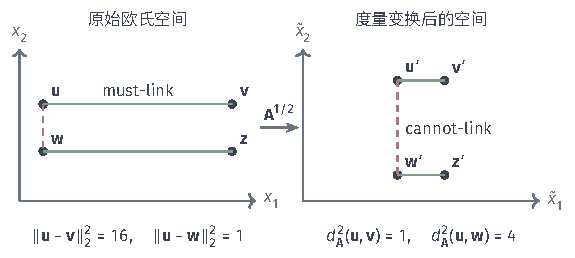
\includegraphics[width=97.331mm]{figures/04-classic-models/00-shared/tikz/clustering-metric-constraints/figure.pdf}
  \caption{度量如何改变成对关系的几何表达。四点为 $\bm{u}=(-2,0.5)$、$\bm{v}=(2,0.5)$、$\bm{w}=(-2,-0.5)$、$\bm{z}=(2,-0.5)$。实线连接 must-link 对，虚线连接 cannot-link 对。这里人为设定 $\bm{A}=\operatorname{diag}(1/16,4)$；右图的距离等于左图的 Mahalanobis 距离，不表示一次真实训练的结果。}
 \label{fig:clustering-metric-constraints}
\end{figure}

记在该度量下全数据的最大距离平方为
\[
 D_k=\max_{p,q\in\{1,\ldots,n\}}
 d_{\bm{A}_k}^2(\bm{x}_p,\bm{x}_q).
\]
对违反 must-link 的样本对，惩罚同时作用于两端所属簇；对违反 cannot-link 的样本对，惩罚其相对于本簇度量下最远样本对的接近程度。具体写为
\begin{align}
 f_M(i,j)
 &=\frac12\left[
 d_{\bm{A}_{c_i}}^2(\bm{x}_i,\bm{x}_j)
 +d_{\bm{A}_{c_j}}^2(\bm{x}_i,\bm{x}_j)\right]
 \mathbb{1}\{c_i\ne c_j\},\nonumber\\
 f_B(i,j)
 &=\left[D_{c_i}
 -d_{\bm{A}_{c_i}}^2(\bm{x}_i,\bm{x}_j)\right]
 \mathbb{1}\{c_i=c_j\}.
 \label{eq:clustering-mpck-penalty}
\end{align}
因此 cannot-link 惩罚非负，must-link 惩罚也不因交换样本对的书写顺序而改变。总目标为
\begin{equation}
 \begin{aligned}
 J={}&\sum_{k=1}^K\sum_{i\in C_k}
 \left[d_{\bm{A}_k}^2(\bm{x}_i,\bm{\mu}_k)
       -\log\det\bm{A}_k\right]\\
 &+\sum_{(i,j)\in M}w_{i,j}^{M}f_M(i,j)
  +\sum_{(i,j)\in B}w_{i,j}^{B}f_B(i,j).
 \end{aligned}
 \label{eq:clustering-mpck}
\end{equation}
权重均非负，每个无序约束对只计一次。负对数行列式阻止特征值趋零，但不能单独阻止矩阵某些方向无限放大；数据退化时仍需约束或正则。

\subsubsection{参数学习}

固定中心和度量时，对一个样本的各簇候选计算完整目标变化，包括几何、行列式及所有相关关系惩罚，再接受不增目标的变更。由于关系项耦合样本，单独比较到中心的距离不足以完成这项选择。

固定分配和度量时，约束项不含中心。对中心求导给出
\[
 2\bm{A}_k\sum_{i\in C_k}(\bm{\mu}_k-\bm{x}_i)=\bm{0},
 \qquad
 \bm{\mu}_k=\frac{1}{|C_k|}\sum_{i\in C_k}\bm{x}_i.
\]
同一簇共用的$\bm{A}_k$在驻点方程中消去，中心因而取普通簇内均值。若需按样本重要性加权，还要在目标中另加相应权重。

度量步可借助散布矩阵理解。令 $\bm{S}_k=\sum_{i\in C_k}(\bm{x}_i-\bm{\mu}_k)(\bm{x}_i-\bm{\mu}_k)^\top$。在固定当前最远样本对、且该样本对在更新后仍保持活跃的一个分支上，约束项写成 $\operatorname{tr}(\bm{A}_k\bm{P}_k)$，其中 $\bm{P}_k$ 汇总违反 must-link 的半权重差分外积，以及违反 cannot-link 的“最远对外积减约束对外积”。于是子目标为
\[
 \operatorname{tr}\bigl(\bm{A}_k(\bm{S}_k+\bm{P}_k)\bigr)
 -|C_k|\log\det\bm{A}_k.
\]
若 $\bm{S}_k+\bm{P}_k\succ0$ 且 $|C_k|>0$，其无约束驻点为
\begin{equation}
 \bm{A}_k=|C_k|(\bm{S}_k+\bm{P}_k)^{-1}.
 \label{eq:clustering-mpck-metric}
\end{equation}
这个驻点式适用于正定的调整散布及保持活跃的最远对分支；更新后需再次核对这两个条件。

保留 $D_k$ 对 $\bm{A}_k$ 的真实依赖时，它是有限个线性函数的最大值，故固定分配和中心的度量子问题是凸的，但通常分段光滑。可在 $\alpha\bm{I}\preceq\bm{A}_k\preceq\beta\bm{I}$、$0<\alpha<\beta$ 的固定域上求解，或使用保持正定且实际下降的优化步骤。对角度量进一步减少参数与矩阵计算。

各步在同一有下界的目标上不增，可推出目标值收敛。度量属于连续参数，即使簇分配不再变化，它也可能继续更新；有限分配数因此不足以证明有限轮停止。实际终止可结合目标和参数变化的容差，并明确空簇处理。

\subsubsection{理论分析}

\paragraph{表达能力}
学习度量能让不同方向采用不同的距离权重。例如，图\ref{fig:clustering-metric-constraints}中的固定矩阵让同一水平行的距离变小、上下两行的距离变大，因而可以保留由行位置决定的关系。若全部簇共享一个正定矩阵，坐标变换仍是可逆线性变换，最近中心区域仍由半空间形成，不能单靠这种共享度量解决完整同心圆的分组。

每簇不同的矩阵增加了另一种表达。冻结参数、按目标的单点几何项比较新点时，得分为
\[
 s_k(\bm x)=(\bm x-\bm\mu_k)^\top\bm A_k(\bm x-\bm\mu_k)
            -\log\det\bm A_k.
\]
两簇的得分差是二次函数，可以形成原空间线性中心无法表达的边界。取二维$\bm\mu_1=\bm\mu_2=\bm0$、$\bm A_1=4\bm I$、$\bm A_2=\bm I$，得分差为$3\lVert\bm x\rVert_2^2-\log16$。选择较小得分会按半径$\sqrt{\log16/3}$分开内外区域，因而能够准确区分半径为$1/2$和2的两圈。这个教学例说明候选增加了什么，并未保证少量关系监督能估计出这组参数。一般多弯曲分组也未必能用固定的两条二次得分表示；成对惩罚对训练对象的作用仍需另外计算。



\paragraph{收敛性}
若把中心限制在有界闭球内，并要求$\alpha\bm I\preceq\bm A_k\preceq\beta\bm I$、$0<\alpha<\beta$，连续参数域紧致；分配只有有限种，目标连续，故全局最小值存在。每一步若在同一目标上不增，目标值便收敛。连续度量仍可能无限次更新，因而有限分配数不能推出有限轮停止，也不能仅从目标值收敛推出参数达到驻点。固定分配和中心的度量子问题为凸问题，但交替求解整体仍非凸，没有上述条件自动给出的全局最优速率。

\paragraph{泛化性}
\begin{theorem}[MPCK-means在有界度量与独立验证下的期望几何风险界]
冻结参数后，采用前面定义的最小得分$\min_k s_k(\bm x)$评价新点。若$\lVert\bm X\rVert_2,\lVert\bm\mu_k\rVert_2\leq r$且各度量特征值位于$[\alpha,\beta]$，则该得分位于$[-d\log\beta,4\beta r^2-d\log\alpha]$，区间长度为$B=4\beta r^2+d\log(\beta/\alpha)$。对独立的$m$个同分布验证样本，以至少$1-\delta$的概率，
\[
 R=\mathbb E\min_k s_k(\bm X)
 \leq\frac1m\sum_{i=1}^m\min_k s_k(\bm X_i^{\mathrm{val}})
       +B\sqrt{\frac{\log(1/\delta)}{2m}}.
\]
\end{theorem}

这是有界损失的单候选Hoeffding结论。它控制冻结度量在新点上的几何得分，不包含未观测样本对的约束惩罚；后者还需规定新关系如何生成和评价。

\subsubsection{优化计算能力}

Xing 等通过相似与不相似样本关系学习 Mahalanobis 度量\scite{clust-xing2003}。这是先单独学习共享度量、再交给聚类算法的解耦方式。这样可以复用监督得到的几何结构，但共享度量仍假设所有簇使用同一种空间变换，后续算法也须与该度量兼容。

\subsubsection{小结}

MPCK-means让关系监督同时改变分配与比较几何，适合距离本身没有反映领域关系的情形。每簇独立度量增加了可调整的方向与尺度，也增加矩阵求解及监督需求；共享或对角形式减小这份负担，同时限制不同群组采用不同几何的能力。

监督还可以在另一个环节发挥作用：先单独学习共享度量再聚类，或修改关系图再求谱表示。这些路线没有联合优化MPCK的完整目标，后续分配也未必逐项满足输入关系。应按关系覆盖、错误类型及新点用途选择监督进入的位置，并检查额外参数是否得到足够支持。

\subsection{模型对比与总结}

关系和种子可以在不同环节减少无标签分组的歧义。COP-K-means直接排除违反must-link或cannot-link的分配，适合可靠且可满足的关系；关系相互冲突时，它可能没有可行结果。软约束改用违反代价保留可行搜索，但权重决定愿意付出多少距离损失来满足监督。Seeded K-means主要用标注记录确定初始中心，Constrained K-means还限制这些记录的后续归属，二者对标签的使用强度不同。

若原始距离本身不能体现监督关系，只限制分配仍会让几何与标签相互拉扯。MPCK-means让每簇度量与分配共同调整，允许不同群组采用不同方向和尺度；共享度量学习减少参数并可复用于其他算法，却要求所有群组接受同一变换。监督也可以直接改变谱图边权，但这会改变图偏好，并不逐项保证最终标签满足关系。

这些方法分别改变可行集合、初始化、几何或图关系。选择前要判断信号是否可靠、覆盖了哪些群组，以及额外度量参数是否有足够监督支持。报告几何目标和关系违反可以解释监督怎样进入拟合，独立参考标签或下游任务再检查这些改变是否带来预定用途。

\section{本章小结}
\label{sec:clustering-summary}

聚类通过结构假设定义群组。原型限定中心周围的相异度，邻域和图限定连接，网格与子空间限定相关区域，层次限定嵌套关系，概率模型限定生成成分。关系与种子监督再减少其中部分歧义。

算法求解与群组用途需要不同证据。目标下降和停止支持计算解释，训练外量化、密度、语义或决策结果支持使用结论；稳定性及零模型补充结构检验。粒度由$K$、密度阈值、带宽、截线或先验控制，均需随任务选择。

评价应先对应群组用途。留出量化误差检验数值压缩，预测对数密度检验生成拟合，独立参考标签检验指定语义，相对无聚类基线的下游损失检验使用收益。\term{轮廓系数}（silhouette coefficient）比较同簇与其他簇的距离，偏好相应的紧凑几何；\term{调整兰德指数}（adjusted Rand index, ARI）比较两份划分的共簇关系，并校正指定随机基准下的一致性\scite{clust-rousseeuw1987,clust-hubert1985}。它们提供不同证据，不能彼此替代。

为检查训练外的用途，可将数据分为\term{发现数据}（discovery data）与\term{验证数据}（validation data）。表示、尺度、相异度、候选和超参数在发现数据上确定，再冻结分配、匹配及指标规则用于验证；时间、地点或个体相关记录按未来使用单位隔离\scite{clust-ullmann2022}。稳定性检验扰动后的重复性，零模型检验结构是否超出指定基线；模拟比较需重跑完整发现流程，把选择过程也纳入基线。

第\ref{chap:dimensionality-reduction}章将学习低维表示，这会同时改变距离、密度和邻接。可视化提供探索线索，群组判断仍需在原始或经验证的表示上取得与用途对应的证据。

\paragraph{扩展阅读}
进一步阅读可围绕同一数据问题，分别写出几何分组与概率成分的定义、学习目标和新样本评价，比较不同假设怎样改变最终群组\scite{bishop2006,hastie2009}。
